\documentclass[12pt]{article}
\usepackage{graphicx,amssymb,amsmath,setspace,comment,verbatim,titling,pgf,lscape}
\usepackage[left=2cm,right=2cm,top=2.5cm,bottom=2cm]{geometry}
\usepackage[round]{natbib}
\usepackage{hyperref}
\usepackage{array}
\usepackage{bbm}
\usepackage{csquotes}


\usepackage[justification=centering]{caption}
\newcommand{\deriv}[2]{\frac{\mathrm{d}#1}{\mathrm{d}#2}}
%%\usepackage{breqn}
\newcommand{\pderiv}[2]{\frac{\partial#1}{\partial#2}}
%\usepackage{siunitx}
\newcolumntype{P}[1]{>{\raggedright\arraybackslash}p{#1}}
\hypersetup{colorlinks,%
						citecolor=black,%
						filecolor=black,%
						linkcolor=black,%
						urlcolor=blue,%
						}


\setlength{\droptitle}{-50pt}

\begin{document}

\title{Hospital Pricing and Public Payments}
\author{%
  Michael Darden, Ian McCarthy, and Eric Barrette\thanks{Darden: George Washington University. McCarthy: Emory University and NBER. Barrette: Health Care Cost Institute.  Correspondence: \href{mailto:darden@gwu.edu}{darden@gwu.edu}; \href{mailto:ian.mccarthy@emory.edu}{ian.mccarthy@emory.edu}; \href{mailto:ebarrette@healthcostinstitute.org}{ebarrette@healthcostinstitute.org}.  We thank Michael Richards, David Dranove and seminar participants at Johns Hopkins University, The Southeastern Health Economics Study Group, George Washington University, The Carey School of Business at Johns Hopkins University, and the Federal Trade Comission.  Finally, we acknowledge the Health Care Cost Institute (HCCI), along with companies providing data (Aetna, Humana, and UnitedHealthcare) used in this analysis.}
}
\date{April 2018}

\maketitle

\begin{abstract}
A longstanding debate in health economics and health policy concerns how hospitals adjust prices with private insurers following reductions in public funding. A common argument is that hospitals engage in some degree of ``cost-shifting,'' wherein hospitals increase prices with private insurers in response to a reduction in public payments; however, evidence of significant cost-shifting is mixed, and the rationale for such behavior is unclear.  We enter this debate by examining plausibly exogenous variation in Medicare payment rates generated by two policies under the Affordable Care Act: the Hospital Readmission Reduction Program (HRRP) and the Hospital Value Based Purchasing (HVBP) program.  We merge rich hospital-level information to actual private-payer payment data from a large, multi-payer database. Our data include roughly 50\% of inpatient prospective payment hospitals in the United States from 2010 to 2015. We find that hospitals that faced net payment reductions from HRRP and HVBP were able to negotiate 1.4\% higher average private payments - approximately \$167 extra for the average acute care claim, or \$183,700 per hospital, based on an average relative reduction in Medicare payments of \$271,000. We find the largest increases in payments for circulatory system (1.9\%) and nervous system (2.1\%) claims.  We also find that cost-shifting is more pronounced in hospitals that serve a higher share of private patients and that are vertically integrated with a physician practice; we find little evidence that our results are driven by policy-induced quality improvements.  Finally, we show that our results are consistent with a model in which hospitals maximize utility as a function of profits, so long as the utility function is concave in profits.
\end{abstract}
\noindent \textit{JEL Classification:} I11; I18; L2 \\\\
\noindent \textit{Keywords:} Hospital Behavior; Healthcare Prices; Medicare Payments; Cost-Shifting; Affordable Care Act\\\\
\setstretch{1.3}

\newpage
\section{Introduction}
A longstanding debate in health economics and health policy concerns a hospital's response to public payment reductions. Two predictions are posited in the literature: 1) standard economic theory for a profit-maximizing firm with market power predicts that a reduction in public payments should put downward pressure on hospital prices as hospitals attempt to attract a larger share of private insurance patients; and 2) an alternative argument, termed ``cost-shifting'' and formalized in \cite{dranove1988}, is that hospitals pass public payment cuts to privately insured patients by negotiating for higher payments from private insurance companies. These arguments offer opposite predictions in terms of changes to hospital prices following a reduction in public payments. Identifying when, if at all, cost-shifting occurs is therefore critical to understanding the effects of future public payment reductions and in guiding future health policy more generally.

Insurance companies have long maintained that Medicare in particular is not paying its fair share \citep{frakt2011}; hospitals often acknowledge cost-shifting when arguing for higher public payments; and the assumption of cost-shifting as common hospital practice is ubiquitous in health care policy debates. For example, in the debate over the Affordable Care Act, President Obama said:
\begin{quote}
\textit{``You and I are both paying 900 bucks on average - our families - in higher premiums because of uncompensated care.''\footnote{For additional examples, see the many excerpts in \cite{dranove2017}, including additional statements from President Obama and the U.S. Supreme Court regarding the Affordable Care Act.}- Barack Obama}
\end{quote}
There is some empirical evidence to support the notion of cost-shifting. Studying California hospitals from 1993-2001, \cite{zwanziger2006} estimate large effects on private payments due to reductions in Medicare and Medicaid payment rates, mirroring the findings of \cite{lee2003}, \cite{zwanziger2000}, and \cite{cutler1998costshift}. \cite{zwanziger2006} estimate that cost-shifting can explain 12.3\% of the total increase in private payers' payments from 1997 to 2001.  Yet, in a systematic review of the literature, \citet{frakt2011} concludes that cost-shifting, if it exists, is not widespread and is not a main driver of increased health care costs.  Indeed, while a simple model of monopoly pricing with price discrimination would suggest different prices for public and private patients \citep{hay1983}, that model would also suggest a \textit{decrease} in the private price for a decrease in public payments.  Furthermore, among both for-profit and non-profit firms, it is unclear why a hospital with the power to raise prices would not have already done so.\footnote{Several papers find zero or even negative price effects following public payment cuts. \cite{white2013} examines market level pricing from the Truven MarketScan data and finds that private prices decrease following reductions in Medicare payment rates. Exploiting a change in Medicaid payment policies in California, \citet{dranove1998} similarly found little evidence of cost-shifting. More recently, using the 2008 stock market collapse as an exogenous change to hospital endowments, \cite{dranove2017} find that the average hospital does not appear to cost-shift, with some evidence of cost-shifting among hospitals with sufficient market share.}

We enter the cost-shifting debate by exploiting the 2013 adoption of the hospital readmission reduction program (HRRP) and hospital value-based purchasing program (HVBP), which are both components of the Affordable Care Act's (ACA) cost containment strategy and which both serve as plausibly exogenous changes in Medicare payment rates.  Initially, the HRRP penalized hospitals for which 30-day readmissions for acute myocardial infarction (AMI), heart failure (HF), and pneumonia (PN) exceeded risk-adjusted thresholds constructed as a function of national averages.  Starting in Fiscal Year (FY) 2013 (October 2012-September 2013), hospitals faced a maximum cut in Medicare payments of 1\% across all Diagnosis Related Groups (DRG); the maximum potential penalty increased to 3$\%$ by 2015.  The \cite{cbo2010} estimates that HRRP will reduce hospital payments from Medicare by \$113 billion through 2019.  By contrast, starting in FY 2013, HVBP reduced Medicare payments to all hospitals by 2\%, but it rewards hospitals with incentive payments for their quality of care over a variety of quality domains. As a result of these potential rebates, hospitals have the opportunity to receive a net payment increase if the rebates exceed the initial 2$\%$ reduction.

An important contribution of our paper is that we tie the variation in public payments created by these policies to data on actual payments from private insurance firms to hospitals.\footnote{Throughout, rather than use the term ``price,'' we refer to the financial transfer for a given procedure as the ``payment'' from a private insurance firm to a hospital.  A payment is distinctly different than a hospital ``charge,'' which effectively represents a hospital's list price for a give procedure. Private insurance firms negotiate substantial discounts from charges.}  Our data, maintained by the Health Care Cost Institute (HCCI), contain all claims made for acute care hospital admissions to three national commercial insurers. \cite{cooper2015} also uses HCCI data to examine broad trends in hospital pricing from 2007 through 2011, but to our knowledge, we are the first to use actual hospital-level payment data in a study of cost-shifting. These unique data include payments for every claim, which capture the negotiated payments between hospitals and insurers and which may differ substantially from charge-based estimates of payments often used in the literature \citep{dafny2009,dranove2017}. Indeed, in our data, the correlation between actual payments and a payment proxy estimated from the Healthcare Cost Report Information System (HCRIS) is 0.435, suggesting that charge-based estimates of payments may contain significant measurement error.  Furthermore, with payment data and a balanced panel of hospitals, we are able to investigate the extent to which hospital fixed effects adequately control for the mean payment to charge ratio within a hospital in a model of log charges \citep{cutler2000}. Our private insurance payment data cover approximately 28\% of individuals under the age of 65 who have employer-sponsored insurance (ESI). When merged with several other datasets on hospital characteristics and HRRP/HVBP penalties, our final analytic data constitute a balanced panel of 50\% of all inpatient prospective payment hospitals in the United States between 2010 and 2015.

Because payment changes under HVBP may be positive or negative (as opposed to HRRP, which are always zero or negative), we calculate the total change in payments from both policies and construct a binary variable that equals one if the net change is negative.  Our baseline empirical specification is a hospital fixed effects estimator in which we estimate the difference in average payments between those hospitals with a net penalty under the HRRP and HVBP relative to those not penalized before and after 2013. Our results reveal an increase in average payments of 1.4\% for penalized hospitals, equivalent to a roughly \$167 increase at the mean from 2013 through 2015. Event study analyses suggest that the effect of a penalty on payments increases over time, likely due to the persistent nature of penalties and the timing between exposure to a penalty and the renegotiation of existing contracts.  While we find some evidence that penalty size matters with respect to price changes, our main results are largely on the extensive margin. Consistent with payment reductions, we find that penalized hospitals decreased Medicare discharges by 2.7\%, while estimated changes in discharges for all other patients (non-Medicare and non-Medicaid) were small and insignificant. As a back-of-the-envelope calculation, our estimated increase of 1.4\% roughly equates to a total increase in private payments of \$183,700 per hospital, based on an average relative reduction in Medicare payments of \$271,000.

Our results are unbiased if there are no unobserved, time-varying factors that influenced payments that were also correlated with penalty status.  While we cannot directly test this assumption, three facts provide supporting evidence for a causal interpretation of our results.  First, the quality metrics that enter into the construction of the HRRP and HVBP adjustments in a given year are calculated based on data from the previous three years.  Thus, between 2013-2015, our net penalty variable was largely pre-determined.  Even still, a competing explanation for our results may be that hospitals penalized under the HRRP and HVBP may have been able to negotiate higher private prices not because of penalties, but because of anticipated differential impacts of the full ACA;\footnote{There is evidence that hospitals located in low-SES areas were more likely to be penalized under HRRP, despite risk-adjustment at the patient level.} however, controls for whether a hospital operates in a state that expanded Medicaid, as well as the inclusion of county fixed effects, do not change our main results. Second, we demonstrate that allowing trends in payments to vary by whether a hospital ever experiences an HRRP/HVBP payment reduction does not significantly change our conclusions. Finally, our results are robust to variety of specification checks, including dropping fiscal year 2012, when the policies affected only a subset of hospitals.  We also demonstrate that our results were unlikely to be caused by vertical integration induced by policy.  Collectively, our baseline results provide support for the notion of some cost-shifting in the modern health care environment, equivalent to as much as a 68 cent increase in private payments for a \$1 decrease in public payments; however, this effect is likely specific to the HRRP/HVBP and should not be directly extrapolated to other Medicare policies. We instead interpret our result as demonstrating the potential unintended consequences of relatively blunt pay for performance programs applied to a heavily concentrated industry.

Because theoretical predictions suggest that profit-motivated (and risk-neutral) firms are unlikely to cost-shift \citep{hay1983}, economic rationales for cost-shifting have focused on a hospital's objective function.  \cite{dranove1988} models a hospital as a utility maximizer, where utility is defined over both profit and quantity.  A hospital may directly value quantity of care for reasons of altruism or prestige, or simply because a non-profit hospital must provide some form of ``community benefit'' to maintain its tax-exempt status.\footnote{The Congressional Budget Office defines community benefits as services geared toward ``promoting the health of any broad class of persons'' \citep{cbo2006}.}  Thus, if cost-shifting exists, evidence is anticipated to be isolated primarily among non-profit hospitals. We embed the model of \cite{dranove1988} within a bargaining model \citep{ho2017} and show that cost-shifting can be predicted for any hospital with diminishing marginal utility of profits. A risk-averse hospital, for example, would still be predicted to cost-shift even if they are otherwise for-profit. When we break our analysis by profit status, we find no economically meaningful difference in effects among for-profit and non-profit hospitals, although our estimates are only significantly different than zero in the case of non-profits.

In a bargaining context, the mechanism for cost-shifting in response to \textit{penalties} incurred from lower-than-expected quality is particularly unclear. How can a penalty for low quality enable a hospital to negotiate a higher payment? We argue that three potential scenarios may allow for such an outcome: 1) if the quality information revealed by the penalty is not new information or is sufficiently noisy, then the penalty is simply a reduction in public payment and the underlying source of the penalty is irrelevant; 2) if the information is new and meaningful, hospitals may exploit the penalty in other service areas (i.e., those not tied to quality scores) where they have a comparative quality advantage in the market; or 3) hospitals with a sufficient bargaining position may be able to translate public payment reductions into higher private insurance payments regardless of a negative quality signal. To demonstrate the potential for cost-shifting in our setting, we address each of these scenarios with a series of alternative specifications and hospital samples.

To address the first scenario, we note that the HRRP and HVBP may not sufficiently discern the true underlying quality of a given hospitals. This follows from the institutional details of the programs (e.g., a hospital must be above or no different than the national average in \textit{all} relevant dimensions in order to avoid a penalty under the HRRP). We attempt to examine this empirically by controlling the overall hospital quality ranking given annually by Hospital Consumer Assessment of Healthcare Providers and Systems (HCAHPS). We find no difference in the effect of Medicare payment cuts on private insurance payments when comparing hospitals with identical overall quality rankings relative to omitting this control. We also show that penalized hospitals already displayed relatively high readmission rates prior to the HRRP/HVBP, further suggesting that penalties under the HRRP/HVBP offered little new quality information to commercial insurers.

To address the second scenario, we note that of the three (five in 2015) acute care admission categories affected by the HRRP, hospitals penalized under the HRRP performed better than the national average in at least one area, on average, in each year.  Thus, we construct measures of average payments within specific acute care admission categories and estimate our preferred empirical model separately for each type of admission.\footnote{We identify ``admission categories'' based on the major diagnostic category classifications.}   Our results suggest marked increases in payments for circulatory system (1.9$\%$) and nervous system (2.1$\%$) claims, which suggest that cost-shifting may occur regardless of whether a specialty is directly related to the payment reductions cuts (such as AMI and HF within HRRP).

For the final scenario, given the lack of data on private insurance market shares at a local level, we follow \cite{wu2010} and proxy for hospital bargaining position using the hospital's share of private insurance patients. The intuition is that hospitals with the largest shares of private insurance patients may represent a more important client to private insurers, and hospitals may leverage this power when faced with public payment cuts. Consistent with this intuition, we find larger price increases following a reimbursement penalty in hospitals with a larger share of private insurance patients. We similarly consider a hospital's relationship with its physicians as a potential proxy for bargaining position, where we posit that an integrated salary model (e.g., a vertically integrated hospital/physician system) will tend to increase a hospital's bargaining position relative to other hospitals \citep{lewis2015}. Here, we find larger effects among hospitals that reported an integrated salary model with its physicians prior to 2012.

By definition, cost-shifting requires that the underlying ``product'' provided by the hospital remain unchanged. In other words, estimating an increase in private insurance prices following a reduction in public payments is not enough -- such an increase must come without a change in endogenously chosen attributes of hospital services for which higher payments would be warranted.  Indeed, a simple explanation for our results could be that HRRP/HVBP induced hospitals to improve quality, which was rewarded in higher private payments.  However, the literature on the extent to which these policies improved quality is mixed. While \citet{mellor2016} finds that HRRP caused a decline in AMI 30-day readmission rates, new evidence from \citet{Ibrahim2017} suggests that observed decreases in readmissions may have been overwhelmingly driven by hospitals coding patients more severely and not by ``real'' quality improvements. There is also some evidence that the HRRP may have decreased readmissions while potentially increasing mortality \citep{gupta2017}.

Another way in which the hospital ``product'' could have changed is by changing the intensity of treatment (i.e., penalized hospitals may do more or less in a given inpatient stay). When we treat average length of stay as a dependent variable, we find little evidence that a net penalty caused hospitals to keep patients longer. We similarly find no significant effects on DRG weights, and we find no evidence that penalized hospitals shift resources to more profitable service lines.

Nonetheless, because of the confidential nature of hospital/insurer bargaining, we cannot completely rule out that higher prices for penalized hospitals where due to other, unobserved factors that are correlated with penalties under HRRP and HVBP. However, such factors would have to vary specifically within penalized hospitals over time, and our results are robust to a variety of specification checks.  Finally, our use of actual private insurer payment data demonstrates that measurement error in charge-based payment proxy variables may explain some of the ambiguity in the cost-shifting literature. Taken together, our results demonstrate that an economically significant degree of cost-shifting (but less than dollar-for-dollar) occurred from the HRRP and HVBP.

Following a discussion of the setting and a detailed explanation of each policy in Section \ref{sec:Background}, we present our data, empirical methods, and baseline findings in Section \ref{sec:Empirical}. Section \ref{sec:Ext} considers several extensions and testable hypotheses implied by the standard theoretical model of cost-shifting.  Section \ref{sec:alt} investigates quality improvements as a competing mechanism behind our results, and Section \ref{sec:Conclusion} concludes.

\section{Background}
\label{sec:Background}

\subsection{Existing Evidence of Cost-shifting}
The debate over whether, and the extent to which, hospitals engage in cost-shifting has been ongoing for decades. While private insurers are naturally averse to higher private prices, hospitals have emphasized the need to cost-shift in an attempt to lobby for larger public payments. For example:
\begin{quote}
\textit{``Cost shifts have been a fact of hospital financial survival for decades.... The data show ...  how private payment is a mirror image of public payment over time and that the cost shift occurs. Hospitals must make up for shortfalls through a combination of approaches and cost-shifting is among them.'' -Rich Umbdenstock, Former President and CEO of American Hospital Association}\footnote{\href{http://blog.aha.org/post/costshifting-in-hospitals-}{``Cost-shifting in Hospitals,'' American Hospital Association Blog Post (AHA STAT), March 26, 2015.}}
\end{quote}

The argument that cost-shifting occurs is easily motivated by observed trends.  In 2015, 55 million Americans were enrolled in Medicare, up from 37.5 million in 1995, and from 1980 to 2014, the share of hospital costs attributable to Medicare rose from 34.6$\%$ to 40.2$\%$.  Meanwhile, in 2014, hospitals endured a shortfall of $\$$35 billion in Medicare payments relative to Medicare patient costs, as compared with a $\$$5 billion surplus relative to costs in 1997.  During this same period, patients insured by private payers became increasingly lucrative: in 2014, the payment-to-cost ratio of privately insured patients was roughly 140$\%$.\footnote{All statistics from the American Hospital Association Trendwatch Chartbook, 2016} Consistent with the trend in profitability of private insurance patients to hospitals, average premiums for covered workers with family coverage more than tripled from 1999 through 2017.\footnote{\href{https://www.kff.org/interactive/premiums-and-worker-contributions/?coverageGroup=family}{``Premiums and Worker Contributions Among Workers Covered by Employer-Sponsored Coverage, 1999-2017,'' Kaiser Family Foundation.}}

While the current conditions for cost-shifting appear to be ripe, much of the evidence of significant cost-shifting comes from the 1980s and 1990s.  For example, \cite{cutler1998costshift} studies cost-shifting during the phase-in of Medicare prospective payments during the 1980s, which resulted in an average 2$\%$ per year reduction in Medicare payments.  He found evidence of dollar-for-dollar cost-shifting.  More recently, \cite{zwanziger2006} study the late 1990s and found that, between 1997 and 2001, cost-shifting was responsible for roughly 12$\%$ of the observed increase in total private payer prices.

In contrast, the simplest argument \textit{against} consistent cost-shifting as a significant mechanism in the hospital market is one of basic microeconomics.  A for-profit and risk-neutral firm with market power who sells to two groups should not respond to an exogenous decline in the price to one group by raising prices to the second group.  \cite{hay1983} shows that, even when the government commits to reimbursing the full average cost of Medicare patients, hospitals will: 1) still charge a higher price to privately insured patients; and 2) respond to lower Medicare payments with \textit{lower} private prices.\footnote{\cite{dor1996} demonstrate that payer-specific marginal costs may be evidence of differential treatment by hospitals.}

In spite of the evidence presented by \cite{cutler1998costshift} and \cite{zwanziger2006}, the empirical evidence of cost-shifting is notably weak.  In a 2011 review of this literature, Austin Frakt states:
\begin{quote}
\textit{``In fact, as a whole, the evidence does not support the notion that cost-shifting is both large and pervasive. Instead, it reveals that cost-shifting can occur but may not always do so. When it has occurred, it has generally been measured at a rate far below dollar-for-dollar''}.
\end{quote}

Indeed, numerous studies have found zero or negative overall price effects, including \cite{dranove2008impact}, \cite{wu2010}, \cite{frakt2014}, and \cite{dranove2017}, but potentially important positive price effects for certain subgroups. For example, \cite{wu2010} shows that hospitals with large shares of private patients (relative to Medicare patients) were able to cost-shift following the 1997 Balanced Budget Act, perhaps due to a stronger bargaining position.

We argue that identification of cost-shifting behavior is inherently difficult for three reasons.  First, the hospital market is incredibly complex.  In addition to many different types of payers, the industry is heavily regulated, and policy changes occur frequently.  We study two exogenous sources of public payment variation in which complexity is arguably a benefit to identification -- as discussed below, a common complaint among hospitals prior to the implementation of HRRP and HVBP was that the policies were opaque with respect to the payment reduction calculation.  Furthermore, because payment reductions were based on past quality metrics, hospitals could only hope to influence \textit{future} penalties once the programs were in place. Such a strategy is further complicated by the regular changes introduced to the programs vis-\`a-vis conditions and procedures being evaluated and the formulas by which HRRP/HVBP payments are calculated. Indeed, \cite{friedson2016} find that, within a relatively wide range of the HVBP penalty thresholds, whether a hospital ultimately underperforms in a given metric is largely random. Second, measurement error in private payments may be severe.  Because private payments are typically not observed, many of the referenced papers above must proxy for private payments, often with charges or costs, but we observe the actual dollar amount of payments from three large private insurers to hospitals.  Finally, heterogeneity in hospital responses to public payment cuts may muddle instances of important cost-shifting.  Indeed, as we emphasize below, our bargaining model of hospital payments predicts that cost-shifting will be largest in markets in which a hospital has greater bargaining position.  That is, the market power of a hospital in the provider market must be large relative to the market power of any given insurer in the insurance market.  While our data do not include good measures of insurance market concentration at a local level, we attempt to examine this heterogeneity with a series of alternative specifications and supplemental analyses by hospital payer mix and by different vertical relationships between physicians and hospitals.

\subsection{Policy Environment: HRRP and HVBP}
The adoption of the Medicare prospective payment system (PPS) in 1983, in which Medicare payments changed from pure fee-for-service to a capitated amount for each inpatient stay depending on diagnosis, generated incentives for hospitals to cut ``excessive'' procedures. PPS also created incentives for hospitals to discharge patients quickly.  By 2011, Medicare paid $\$$24 billion per year for 1.8 million hospital \textit{readmissions} -- admissions to any hospital within 30-days of discharge for the same condition.  While some readmissions are unavoidable, the HRRP was a cost containment in the ACA designed to levy penalties on hospitals with ``excessive'' readmissions.  Starting in 2013, hospitals with risk-adjusted readmissions in acute myocardial infarction, heart failure, and pneumonia that exceeded national comparison averages saw overall Medicare payment cuts of up to 1$\%$.   In 2015, the maximum penalty increased to 3\%, total penalties rose to \$420m \citep{rau2015}, and applicable conditions were expanded to include chronic obstructive pulmonary disease and total hip and knee replacements.  Evidence has been suggestive that HRRP has reduced readmissions in the tested conditions.  For example, \cite{mellor2016} found that HRRP was associated with declines in AMI readmission, which were not due to delay of treatment, changes in intensity, or selective patient mix. And \cite{gupta2017} find a 5$\%$ reduction in overall readmissions and 3$\%$ reduction in all-cause mortality, which was mostly driven by quality improvement.

By contrast, the Hospital Value-Based Purchasing (HVBP) program is rooted in a standard principal-agent model in which the principal (CMS in this case) contracts with agents (hospitals) to provide quality care to Medicare enrollees. The HVBP program scores hospitals based on their achievement (comparison to other hospitals) as well as their improvement (comparison to their own previous performance).  Similar to the HRRP, the HVBP bases changes in payments on past quality.  However, unlike the HRRP, the HVBP program is funded by reducing all hospitals' base operating Medicare severity diagnosis-related group (MS-DRG) payments by 2$\%$ and creating rebate incentives depending on defined quality metrics.  The program defines several quality domains and converts measures of quality within each domain to points, which are aggregated and mapped to a total point score.  The total point score determines the magnitude of the payment change, which may be positive or negative depending on if a hospital generates a rebate large enough to offset the 2$\%$ reduction.  Not surprisingly, \cite{norton2017} show that HVBP generated improvements in the specific domains with the highest marginal incentive to improve care.

\section{Empirical Analysis}
\label{sec:Empirical}

\subsection{Data}
Our primary data come from three large health insurance firms that insure roughly 28$\%$ of all individuals under the age of 65 with employer sponsored health insurance over the period of 2010 through 2015.  To these data, we merge information on HRRP and HVBP penalties/rewards and other cost information from the Healthcare Cost Report Information System (HCRIS); hospital-level characteristics such as bed count, for-profit status, and system membership from the American Hospital Association (AHA) annual surveys; data on a hospital's payer mix (i.e., the number and share of Medicare, Medicaid, or private insurance patients) also from HCRIS; and county-level demographic characteristics from the American Community Survey (ACS).  We restrict our sample to community hospitals in urban areas and in the contiguous United States, with at least 30 staffed beds, at least 25 admissions in a given year in the HCCI data, and observed HRRP/HVBP from HCRIS. Our final sample consists of 1,386 hospitals and 8,316 hospital/year observations.\footnote{We also consider alternative samples in which we allow for missing net penalty values from HCRIS or where we arbitrarily set missing HRRP/HVBP values to 0 (e.g., under the assumption that missing values indicate that the hospital was excluded for the program in that year). Results from these samples are provided in the supplemental appendix.}

Because hospital payments are often bundled across services, we follow \citet{gowrisankaran2015}, who use similar payment data from Northern Virginia, and aggregate payments to the hospital level by dividing the total payment for each claim by the appropriate DRG weight and regressing this amount on individual (claimant) and hospital fixed effects.  Using the estimated regression results, we predict the risk-adjusted mean hospital payment for a given year, which reflects the mean bargained payment. Table \ref{tab:summarystats} presents mean payments across hospitals over time. While average risk-adjusted payments received by hospitals increase roughly 5$\%$ between 2010 to 2015, shares of public (Medicare \& Medicaid) and private patients remain relatively stable over time.  Importantly, while shares remain stable, within-hospital patient mix may vary considerably over time as a function of public payments, which is why we treat payer-specific discharges as a separate dependent variable.  The last column of Table \ref{tab:summarystats} shows the fraction of hospitals subject to a net Medicare payment reduction.  Because the CMS fiscal year is from October through the following September, 28$\%$ of hospitals faced a penalty in calendar year 2012 (after October) because of discrepancies between the fiscal year of the hospital and that of CMS.  By 2015, 76$\%$ of hospitals faced some payment reduction. Among those hospitals ever observed to be penalized during our sample period, the overall average penalty amount was \$145,630, which increased from \$129,532 in 2013 to \$224,388 in 2015.


Since our baseline empirical specification depends on within-hospital variation, we split our sample by whether a hospital ever faced a payment reduction under HRRP and HVBP during our sample period.  Table \ref{tab:bypenalty} presents summary statistics of our main dependent variable and some independent variables by ever-penalized status.  Payments to never-penalized hospitals are marginally higher than those to penalized hospitals over the 2010--2015 period.  Non-profit hospitals (public and private) constituted a much larger share of never-penalized hospitals, suggesting that non-profit hospitals may be of higher quality, at least in terms of HRRP and HVBP.  However, case mix is significantly more severe in the ever-penalized hospitals, which suggest that CMS risk-adjustment in HRRP and HVBP may not perfectly adjust penalty thresholds.  Ever-penalized hospitals tend to be in more competitive markets, have lower Medicare share, and come from more heavily populated counties.  Evidence from Table \ref{tab:bypenalty} suggests that controlling for hospital fixed effects is important in models of hospital payments because of persistent differences between ever-penalized and never-penalized hospitals.

The log of the annual, within-hospital mean of private insurance payments constitutes our primary dependent variable of interest. For brevity, we refer to this variable simply as the log mean payment. For comparison with the literature, we also follow \cite{dafny2009} in estimating hospital prices using the average net revenue for non-Medicare inpatient discharges. Specifically, we convert inpatient gross charges to inpatient net revenue by multiplying the hospital's total net revenues by the total gross charge ratio. Payments for Medicare inpatient services are then subtracted from inpatient net revenue to arrive at inpatient revenues from all non-Medicare patients, which we divide by the hospitals' discharges to derive the per-discharge net revenue amount. Since Medicaid revenues are not provided in HCRIS, the measure is a weighted average of net revenue per discharge for commercially insured and Medicaid patients where the weights equal the share of inpatient discharges belonging to each payer. This same measure has been used in recent studies examining hospital pricing behavior, including \cite{schmitt2017} and \cite{lewis2015}. To eliminate outliers, we trim the lower and upper tails at the 5th and 95th percentile of the resulting price distribution, and we normalize this estimated price based on the hospital's observed case mix index (CMI) from the inpatient prospective payment system (IPPS) final rule files. To differentiate this measure of price from our observed payments from the HCCI data, we refer to this measure as the log mean net charge.

Finally, since standard theory of a for-profit firm suggests that the number of public insurance patients decreases following a reduction in the administrative price, we also include measures of payor mix as an additional set of outcomes. These measures include the log number of Medicare discharges, the log number of Medicaid discharges, and the log number of other discharges (non-Medicare and non-Medicaid). We also considered the Medicare, Medicaid, and other insurer shares (rather than log counts). Those results are excluded for brevity but qualitatively similar to the analysis of log counts.

\subsection{Regression Analysis}
Our baseline empirical specification isolates within-hospital variation in private payments over time by whether a hospital faced a net penalty from the HRRP and HVBP. This analysis therefore focuses on the extensive margin of penalties.  Equation 1 presents our main empirical model:
\begin{equation}
\label{eq: reg}
y_{ht} = \alpha_{h} + x^{'}_{ht}\beta + \delta1[Penalty_{t}]  + \theta_{t}  +  \epsilon_{ht},
\end{equation}
where outcome $y_{ht}$ at hospital $h$ in fiscal year $t$ is a function of a hospital specific intercept, $\alpha_{h}$; a vector of time-varying hospital and market-level exogenous characteristics, $x_{ht}$; an indicator for a net penalty under the combination of HRRP/HVBP policies; controls for year effects, $\theta_t$; and an i.i.d. error term $\epsilon_{ht}$.  Because the penalty indicator is zero for all hospitals in 2010 and 2011, and because we include hospital fixed effects, Equation 1 represents an unscaled difference-in-differences estimator. Our parameter of interest, $\delta$, captures the extent to which hospitals penalized under the HRRP/HVBP receive differential private payments relative to hospitals with no penalty.  For a causal interpretation of $\delta$, the underlying assumption in Equation 1 is that there are no time-varying unobserved characteristics that differentially affect payments in penalized hospitals relative to non-penalized hospitals, an assumption that we address in the next subsection.

Table \ref{tab:baselineresults} presents results from Equation 1 for the log of mean payments, the log of mean net charges, and several (logged) payer-specific discharge variables. The first column of Table \ref{tab:baselineresults} demonstrates that hospitals that faced payment reductions increased payments by 1.4\% over the period of 2012-2015.  This represents a roughly \$155 increase in the average payment at the mean payment reported in Table \ref{tab:summarystats}.  Column 2 presents estimates from a similar model in which we replace negotiated payments with the log of mean net charges as discussed previously \citep{dafny2009,lewis2015,schmitt2017,dranove2017}. Results in column 2 suggest a smaller and statistically insignificant change in log mean net charges for penalized hospitals, which we argue demonstrates the importance of using actual payment data.  Columns 3 and 4 of Table \ref{tab:baselineresults} show movement \textit{away} from Medicaid and Medicare patients for penalized hospitals, with discharges decreasing by 4.5\% and 2.7\%, respectively.

To investigate the intensive margin effect of HRRP/HVBP penalties on hospital payments, we calculate the median dollar value of the penalty (bonus) conditional on receiving a penalty (bonus), and we define indicators for whether a hospital has a large or small penalty (bonus).  We substitute three of these indicators into Equation 1 in place of the net penalty indicator, with the omitted category being those hospitals receiving a small bonus.  Results are presented in Table \ref{tab:int}.  Consistent with our results in Table \ref{tab:baselineresults}, we find that average payments are significantly higher in penalized hospitals relative to those receiving a small bonus, but we are unable to statistically separate the effects of a small and large penalty.  Receiving a large bonus is associated with a decrease in average payments, although this effect is not statistically significant and is economically small in magnitude.


Equation 1 exploits within-hospital variation in payments and penalties to identify the average effect, over all years of penalties, of a hospital penalty on average payments.  Given that payments between hospitals and private insurers are renegotiated every one to three years, we expect that the estimated effects should be increasing over time as more contracts are renegotiated.  To investigate, we estimate two event studies, presented in Figure \ref{fig:event}.  Figure \ref{fig:event}a presents event study estimates for each year prior to and after the realization of a penalty.  The omitted category is the year just prior to a penalty, and all binary variables are set to zero for those hospitals never observed to be penalized.  Figure \ref{fig:event}a demonstrates that a penalty first observed in year ``first'' translates to significantly higher payments over time.  However, because penalized hospitals receive their first penalty at different times, estimates increasingly far from the first year of a penalty contain increasingly few hospitals (e.g., the estimate on the binary variable for three years after the penalty is only identified off of hospitals first penalized in 2012).  Furthermore, it is unclear to what extent the positive and significant estimates following a penalty are driven by the initial penalty or by subsequent penalties.  However, Figure \ref{fig:event}a demonstrates a statistically insignificant pre-trend in payments, especially for the bulk of our hospitals one and two years prior to being penalized.

Because of the selection problem in Figure \ref{fig:event}a, we estimate an alternative event study in which we restrict our sample to only those hospitals first penalized in 2012 - the first possible year of a penalty - along with never penalized hospitals.  Figure \ref{fig:event}b presents these results, where the omitted year is 2011.  For these hospitals, payments in 2010 were not significantly different from 2011, but from 2012 through 2015, payments increased in each year.  The growth in payments in Figure \ref{fig:event}b is likely due to both repeated penalties (a penalty is higher persistent over time in our data) and to the fact that more of the treated hospitals were able to renegotiate payments.\footnote{The event study on our full sample that estimates coefficients on one year prior to and in the first year of a penalty yields a positive and statistically significant effect on payments following a penalty, which demonstrates a significant effect even for the fraction of hospitals scheduled to renegotiate payments in the first year of a penalty.}

Taken together, results from Tables \ref{tab:baselineresults} and \ref{tab:int} and Figure \ref{fig:event} suggest meaningful increases in average hospital payments from private payers for those hospitals penalized under the combination of HRRP and HVBP.


\subsection{Robustness}
Results in Table \ref{tab:baselineresults} reflect the causal effects of the HRRP and HVBP penalties if there are no unobserved, time-varying factors that influence our outcomes and are also correlated with penalty status.  While we cannot completely rule out this possibility, we estimate a variety of alternative specifications in order to examine the influence of several potential confounders.  First, we allow the trend in outcomes to vary by whether a hospital is ever-penalized. Differential trends conditional on penalty status and other controls would be suggestive of time-varying unobserved heterogeneity and would generally bias our estimate of $\delta$ towards zero.  These results are summarized in panel 1 of Table \ref{tab:robustness}. The estimate for log mean payments decreases from 1.4\% to 1.0\% when allowing for differential trends, but nonetheless remains economically meaningful and statistically significant. The remaining results are broadly consistent with with Table \ref{tab:baselineresults}. We also present the p-values of a joint test of the null that the time trend dummies between ever-penalized and never-penalized hospitals is the same. For our log mean payment outcome, this test fails to reject the null of common trends between the ever-penalized and never-penalized hospitals (p-value $=$ 0.497). We reject the null in the case of log mean net charges and in the case of log Medicare discharges, which suggests the presence of some time-varying unobserved heterogeneity for these outcomes. This result makes sense given that the net penalty directly affects the Medicare market and therefore also affects our calculation of mean net charges by construction.

Second, we are concerned that unobserved differences across markets (e.g., with regard insurer market power) may influence our estimates. We therefore include a set of county-level fixed effects, with results summarized in panel 2 of Table \ref{tab:robustness}. Here, we continue to find positive and significant effects on private insurance payments, as well as significant reductions in the log number of Medicare discharges. These results suggest that local area variation in provider or insurer markets is not driving our results.

Third, we remain concerned that other changes in the hospital-insurer relationship may drive payments after the full implementation of the ACA in 2015.\footnote{A model in which we dropped 2014 and 2015, relying on only 2013 as our ``post'' period found an estimate of $\delta$ of 0.01, which was not significant.  Given that, to cost-shift, a hospital must renegotiate its payments, we argue that one year after the policy is insufficient to detect a significant effect.  Furthermore, due to the uncertainty in the amount of payment reductions coming from the HRRP and HVBP, we argue that it was unlikely that hospitals anticipated the full payment cut prior to the implementation of HRRP and HVBP.} We therefore consider an alternative specification in which we include an indicator for whether the hospital was in a Medicaid expansion state as of 2014. These results are presented in panel 3 of Table \ref{tab:robustness} and are largely unchanged from our initial estimates.

Fourth, since the HRRP and HVBP are intended to reward and/or punish hospitals based in-part on quality of care, a hospital's ability to translate HRRP and HVBP penalties into higher private insurer payments may depend on whether such penalties reveal new quality information to the market. Existing findings from \cite{dranove2008} and others tend to find relatively small effects of quality reporting on hospital choice. As \cite{dranove2008} state, ``report cards do not always convey `news' about quality; in some cases the rankings confirm with prior beliefs about quality.'' To the extent that penalties from the HVBP and HRRP do not reveal any new information to the market, then the penalty acts simply as a reduction in public payments and the standard arguments for cost-shifting apply. The distribution of readmission rates across hospitals before the HRRP/HVBP suggest this is the case, as penalized hospitals already displayed higher readmission rates relative to other hospitals in the years prior to 2012. These distributions are presented in Figure \ref{fig:pre_readmits}. We also examine this issue with an alternative specification in which we control for a hospital's overall quality as measured by patients' overall hospital rating from the Hospital Consumer Assessment of Healthcare Providers and Systems (HCAHPS).  Panel 4 of Table \ref{tab:robustness} reports results from this model, with estimates almost identical to those in Table \ref{tab:baselineresults}.

Fifth, because of discrepancies in the timing of hospital fiscal years (both across hospitals and with CMS), the exact timing of the realization of Medicare payment cuts varies across our sample. In panel 5 of Table \ref{tab:robustness}, we report results from a model in which we drop fiscal year 2012 from our analysis. Again, our results are similar to those in Table \ref{tab:baselineresults}.

Sixth, it may be that other changes introduced through the ACA (e.g., expansion of insurance on the individual market) may have changed the ``typical'' patient being admitted to the hospital. In panel 6 of Table \ref{tab:robustness}, we demonstrate that our results are again unchanged when conditioning on the hospital's average case mix.

Finally, the novel aspect of our data is that, for a given acute care claim, we observe the actual payment from a private insurer to the hospital. Private insurance payments reflect some endogenously bargained discount on the charge or markup relative to Medicare payment rates and are therefore fundamentally different from charges, which reflect a hospital's list price for a given service. As noted above, the correlation in our data between mean payments and charge-based payments is 0.435, which suggests that measurement error in a model of log mean net charges could be significant. Many studies of hospital pricing proxy for payments with hospital charges and argue that hospital fixed effects control for mean differences between charges and payments \citep{cutler2000}. The last panel of Table \ref{tab:robustness} presents results of Equation 1 without hospital fixed effects for each of our dependent variables.  Estimates of $\delta$ for log mean payments are negative, large, and significant. Relative to our initial results, these findings suggest that: 1) persistent and unobserved hospital-level heterogeneity is an important driver of outcomes in our setting; and 2) hospital fixed effects may in fact go a long way toward controlling for mean differences between charges and payments. However, we emphasize the importance of payment data with respect to the precision and measurement of hospital-insurer bargaining, noting the lack of statistical significance in our model of log mean net charges presented in Table \ref{tab:baselineresults}. Ultimately, these results offer some assurance that findings of a significant effect using charge-based estimates of prices are indeed reflective of a true price increase, while findings of an insignificant effect may be driven by incorrect inference (e.g., due to measurement error) or due to a true underlying null effect.

\section{Heterogeneity in the Extent of Cost-Shifting}
\label{sec:Ext}

\subsection{Theoretical Framework}
As initially examined in \cite{dranove1988}, a hospital may pursue a cost-shifting strategy if the hospital's objective function includes something other than pure profit (e.g., if the hospital receives direct utility from the quantity of services provided). For this reason, cost-shifting is thought to more likely occur among non-profit hospitals, if at all. Indeed, to maintain their tax exempt status, non-profit hospitals are required by the IRS to provide community benefits.\footnote{Of course, this does not mean that non-profit hospitals are fully altruistic. In fact, evidence on non-profit hospital behavior relative to for-profit hospital behavior is mixed. For example, \cite{silverman2004} and \cite{dafny2005} find evidence that non-profits ``upcode'' less frequently, while \cite{gaynor2003} find that non-profit hospitals have lower marginal costs but higher markups than for-profit hospitals.} Since over 80\% of hospitals in our sample are non-profit, this implies that the objective function of the majority of hospitals in our analysis extends beyond pure profit-maximization.  Importantly, the model posited in \cite{dranove1988} assumes that hospitals set payments unilaterally, and it is not immediately clear whether this prediction extends to a modern managed care market in which hospitals and private insurers negotiate over private prices.

To more formally examine the presence of cost-shifting in a bargaining context, we embed the hospital cost-shifting model from \cite{dranove1988} in a hospital-insurer bargaining model similar to that in \cite{ho2017} (HL), \cite{gowrisankaran2015}, \cite{lewis2015}, and \cite{dor2004}. Specifically, we consider a hospital whose objective is to maximize a function of profits and quantity of care provided, denoted by
\begin{equation}
 U\left( \pi_{j} = \sum_{i=1}^{N_{j}} \pi_{i,j}^{h} + \pi_{g,j}^{h}, \sum_{i=1}^{N_{j}} D_{i,j}^{h}, D_{g,j}^{h} \right),
\label{eqn:nfp_objective}
\end{equation}
where $\pi_{j}$ denotes total profits for hospital $j$ and $D_{i,j}^{h}$ denotes hospital demand from insurer $i$. Following HL, we assume $$\pi_{i,j}^{h}=D_{i,j}^{h}(p_{i,j}-c_{i}),$$ where $p_{i,j}$ denotes the negotiated payment between insurer $i$ and hospital $j$. We also follow HL in assuming that patients are ``unaware or unable to determine their [financial] liability prior to choosing their provider.'' In other words, the negotiated payment $p_{i,j}$ does not affect demand for a specific hospital. The subscript $g$ denotes public (or government) insurers, for which the payment is administratively set at $p_{g}$. Finally, again following HL, we assume that profits for insurer $i$ are
\begin{equation}
\pi_{i}^{M} = D_{i} \left( \theta_{i} - \eta_{i} \right) - \sum_{j=1}^{N_{i}} D_{i,j}^{h} p_{i,j},
\label{eqn:ins_profit}
\end{equation}
where $D_{i}$ denotes the number of enrollees for insurer $i$, $\theta_{i}$ denotes the insurer's premiums, $\eta_{i}$ denotes insurer costs per-enrollee other than inpatient hospital care, and $D_{i,j}^{h} p_{i,j}$ reflects payments to hospitals for care provided to the insurer's enrollees.

The negotiated price between hospital $j$ and insurer $i$ is such that
\begin{equation}
 p_{ij}= \arg \max_{p_{ij}} \left(\triangle U_{j} \right)^{b_{j}} \times \left(\triangle \pi^{M}_{i} \right)^{1-b_{j}},
 \label{eqn:neg_price}
\end{equation}
where $\triangle U_{j}$ denotes the change in hospital $i$'s utility from reaching an agreement with insurer $i$, and similarly $\triangle \pi^{M}_{i}$ denotes the change in insurer profits from an agreement with hospital $i$. $b_{j}$ denotes the bargaining weight of hospital $j$, expressed as the weight to which the hospital's payoffs are given in the overall net value.

The first order condition for equation \ref{eqn:neg_price} can be simplified to
\begin{equation}
 b_{j} \triangle \pi_{i}^{M} \pderiv{U_{j}}{\pi_{ij}^{h}} - (1-b_{j}) \triangle U_{j} = 0.
\label{eqn:price_foc}
\end{equation}
Applying the implicit function theorem yields the relevant comparative static:
\begin{equation}
\deriv{p_{ij}}{p_{g}} = \frac{- b_{j} \triangle \pi_{i}^{M} \pderiv{^{2}U_{j}}{\pi_{j}^{2}}D_{g}^{h}}{D_{ij}^{h}\left(b_{j} D_{ij}^{h} \pderiv{^{2}U_{j}}{\pi_{j}^{2}} - (1-b_{j}) \pderiv{U_{j}}{\pi_{j}} \right)}.
\label{eqn:comp_static}
\end{equation}
We can see immediately from Equation \ref{eqn:comp_static} that $\deriv{p_{ij}}{p_{g}}<0$ whenever $\pderiv{^{2}U_{j}}{\pi_{j}^{2}}<0$. This means that hospitals must have some diminishing marginal utility of profits for cost-shifting to occur. Importantly, we obtain a prediction of cost-shifting without hospitals deriving utility from something other than profits, which is necessary for cost-shifting to occur in \cite{dranove1988}. If we interpret diminishing marginal utility simply as a reflection of risk-aversion (e.g., in the context of uncertain demand or uncertain ``exposure'' to the HVBP/HRRP penalties), then this model predicts any risk-averse hospital to potentially cost shift, regardless of whether the hospital is for-profit or non-profit.\footnote{While it is commonly assumed that for-profit firms are risk-neutral, there is an influential literature examining the role of risk aversion in the context of demand uncertainty. See, for example, \cite{sandmo1971}, \cite{holthausen1979}, \cite{mcdonald1985}, \cite{guiso1999}, \cite{chavas1996}, \cite{asplund2002}, and many others. Intuitively, risk aversion could be introduced through the presence of risk-averse shareholders or managers/administrators. In the case of physician-owned hospitals, diminishing marginal utility of profits is analogous to diminishing marginal utility of income to the physicians, since they are the residual claimants for hospital profits.} Our model also predicts that cost-shifting should be largest for hospitals with more bargaining power, $b_{j}$, or a better bargaining position.

\subsection{Heterogeneity by Hospital Objective Function}
To empirically investigate the role of for-profit versus not-for-profit status, we re-estimate Equation 1 separately for non-profit and for-profit hospitals.  The results are presented in Table \ref{tab:byprofit}. Although our estimates among non-profits are more precisely estimated, we otherwise see no meaningful difference in the effects of HRRP and HVBP penalties on the magnitude of cost-shifting between for-profit and non-profit hospitals. In panels 2 and 4 of Table \ref{tab:byprofit}, we allow for differential trends by penalty status (analogous to the overall results in panel 1 of Table \ref{tab:robustness}), again with little change relative to the initial results and panels 1 and 3, respectively.

To the extent that these results reveal information on the underlying objective function of the hospital, out estimates suggest that attitudes toward risk may be similar among for-profit and non-profit hospitals. These findings therefore contribute the broader literature on the theory of the hospital and how, if at all, hospital behaviors differ according to profit status \citep{sloan2001,duggan2002,horwitz2005,horwitz2009,david2009}.

\subsection{Heterogeneity by Bargaining Position}
From Equation \ref{eqn:comp_static}, a hospital's incentive to cost-shift is larger as the insurer's outside option decreases (i.e., $\triangle \pi_{i}^{M}$ increases) and as the number of public-payer patients increases, $D_{g}^{h}$, while the incentive to cost-shift is reduced if the hospital receives a larger number of patients from insurer $i$. Practically, this suggests that hospitals will be more likely to cost-shift if they have some \textit{relative} market power, where the insurer is heavily dependent on the hospital but where the hospital does not receive a large number of patients from any given insurer. In the parlance of \cite{lewis2015}, relative market power describes the hospital's ``bargaining position,'' while a hospital's ``bargaining power'' is reflected by $b_{j}$.\footnote{While bargaining power and bargaining position may seem to be related, \cite{lewis2015} find that bargaining power is not significantly affected by the hospital's bargaining position or direct market share.}

To investigate, we attempt to proxy for a hospital's bargaining position by constructing the quartile of the hospital's share of public patients relative to total patients, and we interact our penalty variable with indicators for each quartile. This analysis is similar to that of \cite{wu2010}, who intuits that a hospital with a large share of private payers represents a more important client for the insurance market, and the hospital may leverage this power when public payments are cut. Applying this intuition to a study of hospital cost-shifting following the Balanced Budget Act of 1997, \cite{wu2010} finds that hospitals with larger shares of private patients were more able to pass Medicare payment reductions on to private payers.

Results are presented in Table \ref{tab:publicshare} and suggest that our initial estimate of cost-shifting is driven by hospitals with the smallest share of public patients. Indeed, the first column of Table \ref{tab:publicshare} demonstrates that payments increased by 3.9\% for hospitals with the smallest share of public patients. This increase was nullified for hospitals in the third and fourth quartile of public patient shares.

Another proxy for bargaining position is whether a hospital is aligned with its network of physicians. \cite{lewis2015}, for example, finds that hospitals that are affiliated with a physician group are able to negotiate a larger share of surplus. Vertical integration with physicians may therefore put some hospitals in a more favorable bargaining position, and thus facilitate a larger increase in private payments, consistent with Equation \ref{eqn:comp_static}. To investigate, we estimate our preferred empirical model on data from only those hospitals that already owned a physician group or physician practice \textit{prior} to 2012.\footnote{The AHA surveys provide information at the hospital-level on whether a hospital currently has an ``integrated salary model.'' This measure unfortunately does not capture \textit{how many} physicians are employed by a hospital, but instead only captures if there is any integrated model reported between the hospital and any of its physicians.} We also estimate our model on hospitals never observed to be vertically integrated.  As shown in Table \ref{tab:VI}, amongst those hospitals already vertically integrated, the effect of a net penalty on payments is 2.3$\%$ and strongly significant; a penalty is associated with a small and statistically insignificant effect on payments among those hospitals never observed to be vertically integrated.\footnote{We also considered whether the penalty itself led to more integrated salary models by treating the binary integration measure as an additional outcome. Here, we estimate a very small and insignificant negative effect of being penalized on the probability of reporting an integrated salary model, suggesting that penalized hospitals were not integrating with physicians due to the penalty. These results are excluded for the paper but available upon request.}

We note that predictions involving a hospitals' bargaining position are less clear when we incorporate the insurer's choice of premiums in the insurance market. If the insurance market is heavily concentrated, then insurers can pass health care price changes on to their plan enrollees \citep{trish2015,ho2017}. This intuition leads to conflicting conclusions: cost-shifting is likely to occur when insurers have a particularly small market share (such that hospitals can leverage their bargaining position), but perhaps also when insurers have a particularly large market share (such that insurers can pass price increases on to plan enrollees). The role of insurance markets on the prevalence or magnitude of cost-shifting is therefore empirically difficult to measure without detailed data on insurance premiums and insurer market shares (at a local level). Because we lack reliable information on local area insurance concentration, we leave as an open question the extent to which cost-shifting is more prominent in markets with both provider market power and a concentrated insurance market.


\subsection{Heterogeneity by Service Area}
As discussed previously, the underlying mechanisms for cost-shifting are unclear in the context of hospital-insurer bargaining. In particular, the reduction in public payments that serve to identify the presence of cost-shifting in our analysis derive from a lower-than-expected performance on some set of quality metrics. For cost-shifting to occur, hospitals must translate this signal into higher prices. We presented evidence in Table \ref{tab:robustness} that our estimates are robust to any reputation effects from the HRRP and HVBP penalties as measured by patients' hospital ratings; however, the quality signal may be uninformative to patients while potentially informative to managed care insurers. In this case, penalized hospitals may instead target other, unrated service areas where they may maintain a comparative quality advantage in the market. To investigate this further, we estimate models of the log of mean payments within acute care admission service categories.

Estimates for $\delta$ are presented in Table \ref{tab:eachcondition} for several categories of acute admissions. For each admission category, we restrict our sample to hospitals with at least 25 admissions in that category in each year of our sample. Table \ref{tab:eachcondition} demonstrates significant increases in payments for nervous and circulatory admissions, suggesting that cost-shifting may occur for multiple types of admissions. Because two of the three original conditions rated by the HRRP (AMI and heart failure) were circulatory system conditions, an open question remains as to how hospitals may negotiate higher prices for these conditions. It could be that the average increase in circulatory system prices is driven by conditions other than AMI or heart failure (e.g., coronary artery disease or stroke), or it could be that the penalty among hospitals that ultimately negotiated higher circulatory system prices was driven by lower-than-expected performance in pneumonia patients rather than AMA or heart failure patients. Because of limited sample sizes for such hospitals and conditions, we cannot examine these questions directly in our data (both due to restrictions on dissemination of small sample size results and due to large variability in prices for infrequent procedures).

\section{Alternative Mechanisms}
\label{sec:alt}
By definition, cost-shifting requires that the underlying hospital ``product'' remain unchanged. To investigate this \textit{ceterus peribus} assumption, we test for disproportionate changes in hospital quality for penalized hospitals.  Since both the HRRP and HVBP are intended to incentivize hospitals to improve quality, a natural question is whether our estimated price increases are simply a reflection of higher hospital quality, for which private insurers should be willing to pay a higher price.  Evidence of such changes may suggest that our estimated price increases are not due to cost-shifting but instead due to a change in endogenously chosen hospital characteristics (which may ultimately lead to a change in negotiated payments).  The existing literature in this area is mixed. \cite{gupta2017} finds that the HRRP did lead to reduced readmissions among heart failure patients but that mortality rates actually increased. \cite{gupta2016}, however, finds some evidence of a reduction in hospital mortality rates (a decrease of about 3\%, significant at the 10\% level) from the HRRP, which may account for as much as 60\% of the reduction in readmissions.  As noted above, \citet{Ibrahim2017} finds that most of the observed reduction in readmissions among penalized hospitals can be attributed to changes in coding practices in which hospitals code patients as more severe.  Regarding the HVBP, the literature generally finds little or no effect on hospital quality \citep{ryan2015,doran2017,norton2017,ryan2017}. Examining data from 2015 to 2016, \cite{norton2017} did find some hospital response to the HVBP, but this response was in specific areas with the greatest marginal revenue rather than those areas with larger quality benefits. Conversely, based on quality data from 2005 through 2014, \cite{gao2015} found no effect of HVBP on quality. \cite{gao2015} also interviewed a handful of hospital officials as part of their analysis. Based on these interviews, the researchers concluded ``the HVBP program generally reinforced ongoing quality improvement efforts, but did not lead to major changes in focus.'' \cite{friedson2016} offer an explanation for these findings, where the authors find that the HVBP does not sufficiently discriminate between hospitals, and whether hospitals are penalized or rewarded by the HVBP program is largely a matter of chance rather than a reflection of true underlying quality.  Existing studies of HRRP/HVBP tend to focus on the Medicare population, but to the extent that HRRP/HVBP may have improved quality of care, such improvements should extend to private insurance patients in order to translate into higher private insurance payments. We are not aware of any evidence in the literature suggesting that quality in the private insurance market improved due to the HRRP or HVBP programs.

Using our data on private payments, we are able to directly address the extent to which hospitals respond to public penalties by reallocating resources towards more profitable services or to improving quality.  Indeed, since our outcome is calculated as an average payment per patient, our results could simply reflect increases in the intensity of treatment, which often serves as a proxy for quality of care.    To investigate, we follow \cite{horwitz2009} in constructing a set of indicators for ``profitable'' (e.g., angioplasty or neonatal intensive care) versus ``unprofitable'' (e.g., alcohol dependency services or hospice care) hospital services.\footnote{A full list of relatively profitable and relatively unprofitable services is provided in Table 2 of \cite{horwitz2009}. Following their analysis, we identify whether a hospital offers these services based on responses from the AHA annual surveys.} We then constructed a ``profitable services index'' calculated as the ratio of profitable services to all profitable and unprofitable services identified by \cite{horwitz2009}. For example, if the hospital offered 2 profitable services and 2 unprofitable services, then the ratio for this hospital would be 50\%. Treating this profitable services index as an additional outcome and repeating our analysis from Section \ref{sec:Empirical}, Table \ref{tab:other_results} demonstrates that we find small and insignificant effects of being penalized. These insignificant effects persist when examining for-profit and non-profit hospitals separately as well as across all robustness checks presented in Table \ref{tab:robustness}.  A similar pattern emerges in Table \ref{tab:other_results} when we consider average length-of-stay and average DRG weights (among our commercial insurance population) as separate outcomes, with insignificant effects of HRRP/HVBP penalties on these outcomes in all specifications considered.  We find little empirical evidence that hospitals increased treatment intensity due to penalties.  These results suggest that hospitals do not respond to HRRP/HVBP penalties by shifting service offerings disproportionately toward more profitable services or by treating patients more intensively.

Indirectly, the results in Table \ref{tab:other_results} support the hypothesis that our estimated increase in payments derives from some underlying increase in actual prices.  Recall that our first robustness check was to flexibly allow the trend in payments to vary by whether a hospital is ever penalized during our sample period.   Along with hospital fixed effects, this differential trends specification controls for time-varying unobserved heterogeneity that is common among penalized hospitals.  As shown in Table \ref{tab:robustness}, allowing for differential trends cuts our estimate in the payment specification by approximately one-third, which may reflect product changes (quality improvements or otherwise) for which high payments were warranted.  However, we emphasize that, even with differential trends, our estimated effect of penalties on payments is still 1$\%$, which is both statistically and economically significant.

\section{Conclusion}
\label{sec:Conclusion}
This paper uses novel payment data from a large, multi-payer database to investigate the extent to which hospitals, faced with public-sector payment cuts, compensate by negotiating for higher payments from private insurers.  We use variation in Medicare payments generated by two cost-containment policies within the ACA -- the hospital readmissions reduction program and the hospital value based purchasing program -- to estimate the role of a net public payment reduction on average hospital payments.  Our results suggest support for a modest degree of ``cost-shifting,''  where the change in payments for hospitals facing a net payment reduction was significantly higher than that for non-penalized hospitals. This qualitative finding is robust to differential time trends among penalized versus non-penalized hospitals, reputation effects as measured by HCAHPS responses, and Medicaid expansion in 2014 as part of the ACA.\footnote{We focus our results on the extensive margin, comparing penalized versus non-penalized hospitals. We also estimated effects on the intensive margin, conditional on hospitals that were penalized in at least one year. We find small and statistically insignificant effects on log mean payments on the intensive margin. Full results from these regressions are available on request.}

Motivated by a simple extension of \cite{dranove1988} to a bargaining framework, we extended our empirical analysis to consider the underlying mechanisms allowing for cost-shifting. First, our theoretical model suggests that cost-shifting will only occur in the presence of diminishing marginal utility of profits, which we argue need not require the hospital to be non-profit. Consistent with this prediction, the magnitudes of our estimates among for-profit and non-profit hospitals are similar; however, our estimates are only statistically significant for non-profit hospitals due to the larger sample size relative to for-profits.

We then considered the mechanisms for cost-shifting specifically in the context of our data. In particular, our empirical analysis identifies cost-shifting from variation across hospitals (on the extensive margin) in penalties levied under the HRRP and HVBP programs. The presence of such a penalty suggests that the hospital has under-performed in some way relative to an average hospital, and it is unclear how a hospital could translate this underperformance into \textit{higher} prices. We intuit two potential mechanisms: 1) by increasing prices for services unrelated to the areas in which the hospital was evaluated and ultimately penalized; and 2) by leveraging its bargaining position as predicted in our theoretical model. We find some evidence in favor of each mechanism, where hospitals do appear to increase prices in areas unrelated to the HRRP and HVBP (but not exclusively in such areas) and where cost-shifting is also largest among hospitals with a more advantageous bargaining position (as proxied by the hospital's share of public insurance patients).

Our initial analysis estimates a 1.4\% increase in private insurance prices for hospitals that were penalized under the HRRP/HVBP programs. Subsequent analysis finds that this estimate is robust to a variety of alternative specifications, and we find no evidence of changes in underlying quality or intensity of treatment. Our estimate implies an increase of \$167 per inpatient stay based on an average private insurance payment of approximately \$12,100 among penalized hospitals. As a back-of-the-envelope calculation, we assume that this payment increase applies to around 1,100 inpatient stays per year.\footnote{Our final price data are based on just over 550 inpatient stays per year per hospital. For purposes of extrapolating the full effect, we assume that our data are reflective of half of the commercial insurance population and that other commercial insurers experienced the same price increase as that estimated from our data.} We therefore estimate a total increase in private insurance payments of up to \$183,700 per hospital per year. To put this in context, penalized hospitals saw an average penalty of around \$205,000, while non-penalized hospitals received an average bonus of just over \$66,000. This yields a differential payment between penalized and non-penalized hospitals of approximately \$271,000. An estimated increase of \$183,700 in private insurance payments therefore translates to cost-shifting at a rate of \$0.68 per \$1 reduction in Medicare payments.

We stress, however, that this amount of cost-shifting follows from a relatively small penalty, and there is intuitively some ceiling by which hospitals will be restricted in their ability to negotiate higher private insurance payments. As the reduction in Medicare payments increases, hospitals are more likely to confront this constraint, at which point the rate of cost-shifting would likely decrease. This intuition aligns with our intensive margin results, where we find that hospitals with very large penalties did not increase private insurance payments any more than hospitals with relatively low penalties. We therefore caution against using this rate of cost-shifting to predict specific commercial insurance payment increases in other contexts.

We also stress that these results should not be interpreted to suggest that pay for performance in healthcare is inherently bad. Instead, we interpret our results as highlighting the importance of how the pay for performance program is designed. In the case of the HRRP, hospitals need only be below average in one area in order to incur some percent penalty levied on all Medicare payments. Most hospitals are not better than average in every dimension, and indeed, as the number of conditions in the HRRP has grown, so too has the percentage of hospitals penalized in a given year (up to 80\% in FY 2015). Intuitively, the HRRP is a relatively blunt instrument that penalizes most hospitals in a given year. Subsequently, HRRP penalties may serve as a poor quality signal. The HVBP may similarly suffer from some basic design problems. For example, in tracking a hospital's performance across 20-plus metrics, it becomes difficult to discern a true quality signal from each hospital. When applied to a highly concentrated private industry, our results suggest that such pay for performance programs may have important unintended consequences.

\newpage
\bibliographystyle{authordate1}
\bibliography{BibTeX_Library}


\clearpage
\newpage
\appendix
\section*{Figures}
\label{app:figures}
\newsavebox{\gfxbox}
\savebox{\gfxbox}{
\centering
\begin{tabular}{cc}
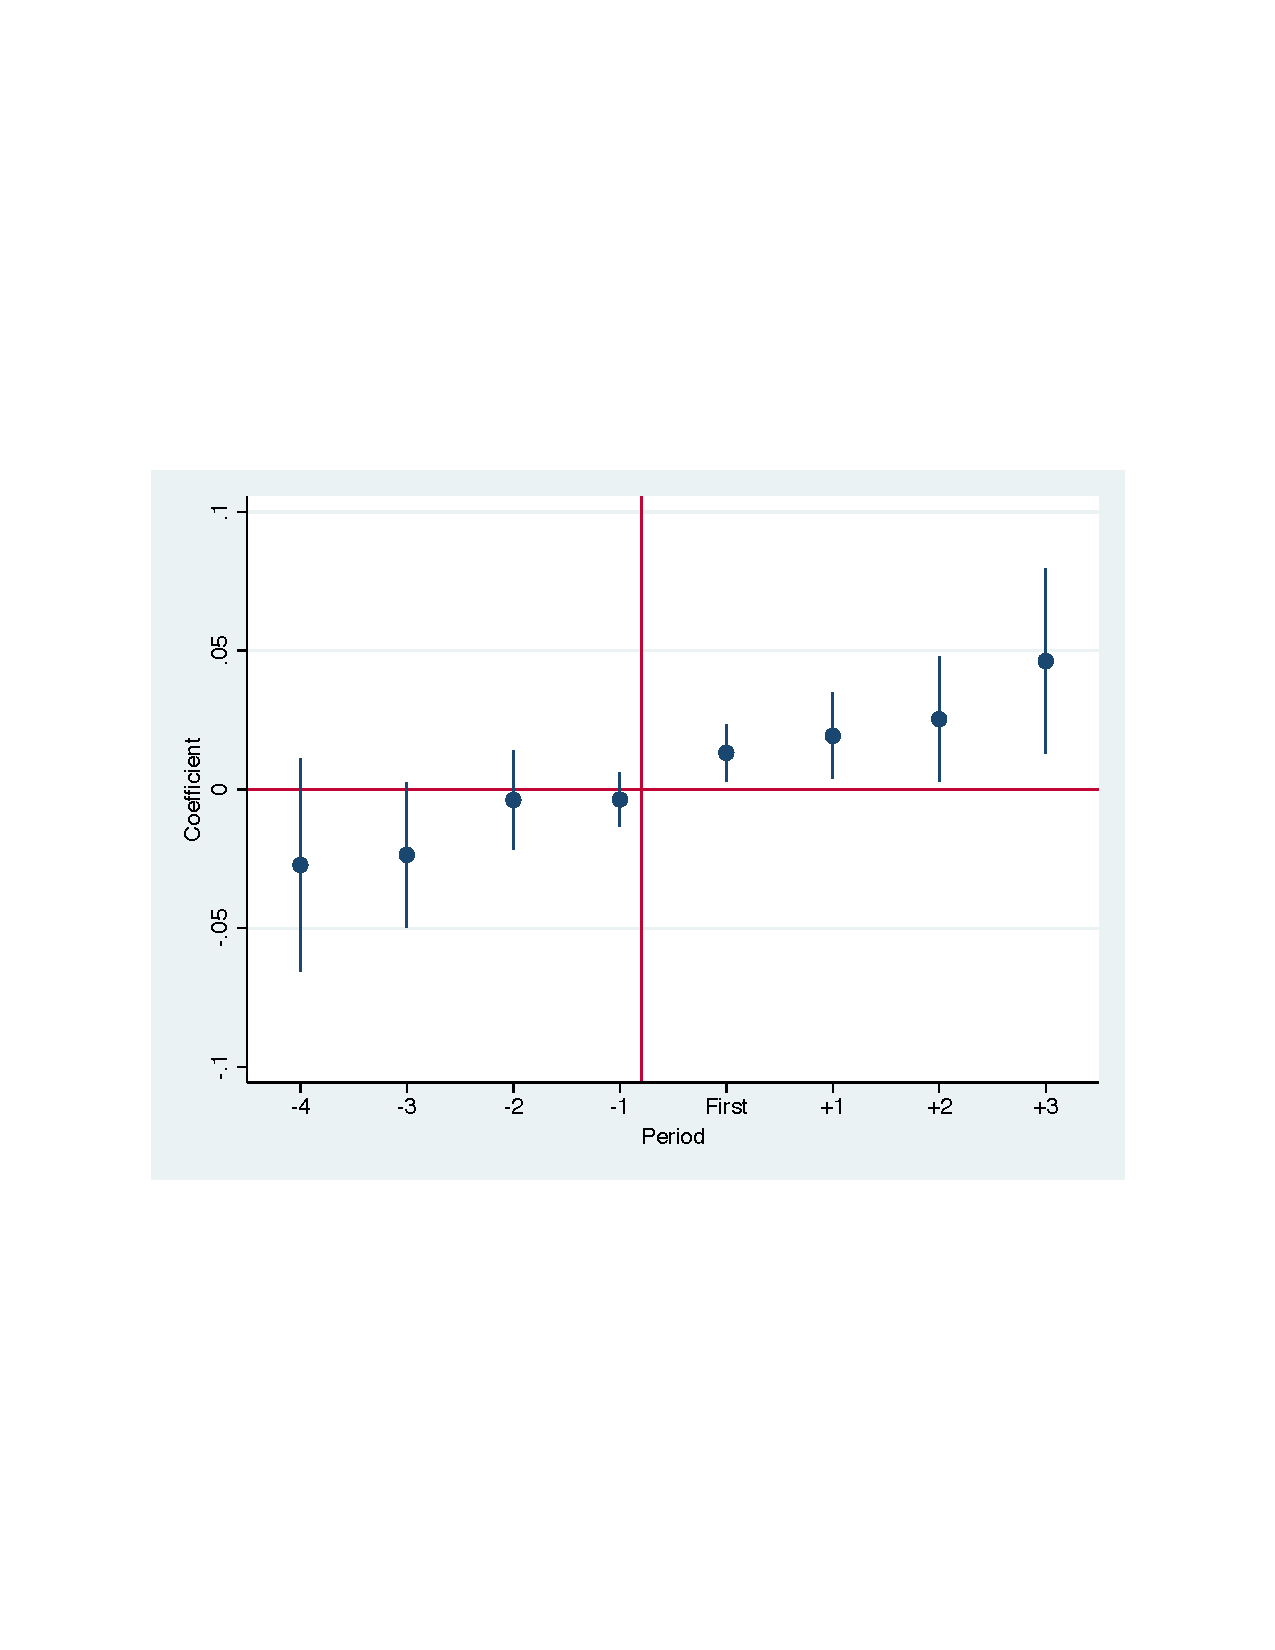
\includegraphics[scale=0.5]{ev_lnprice_hcci_all.pdf} & 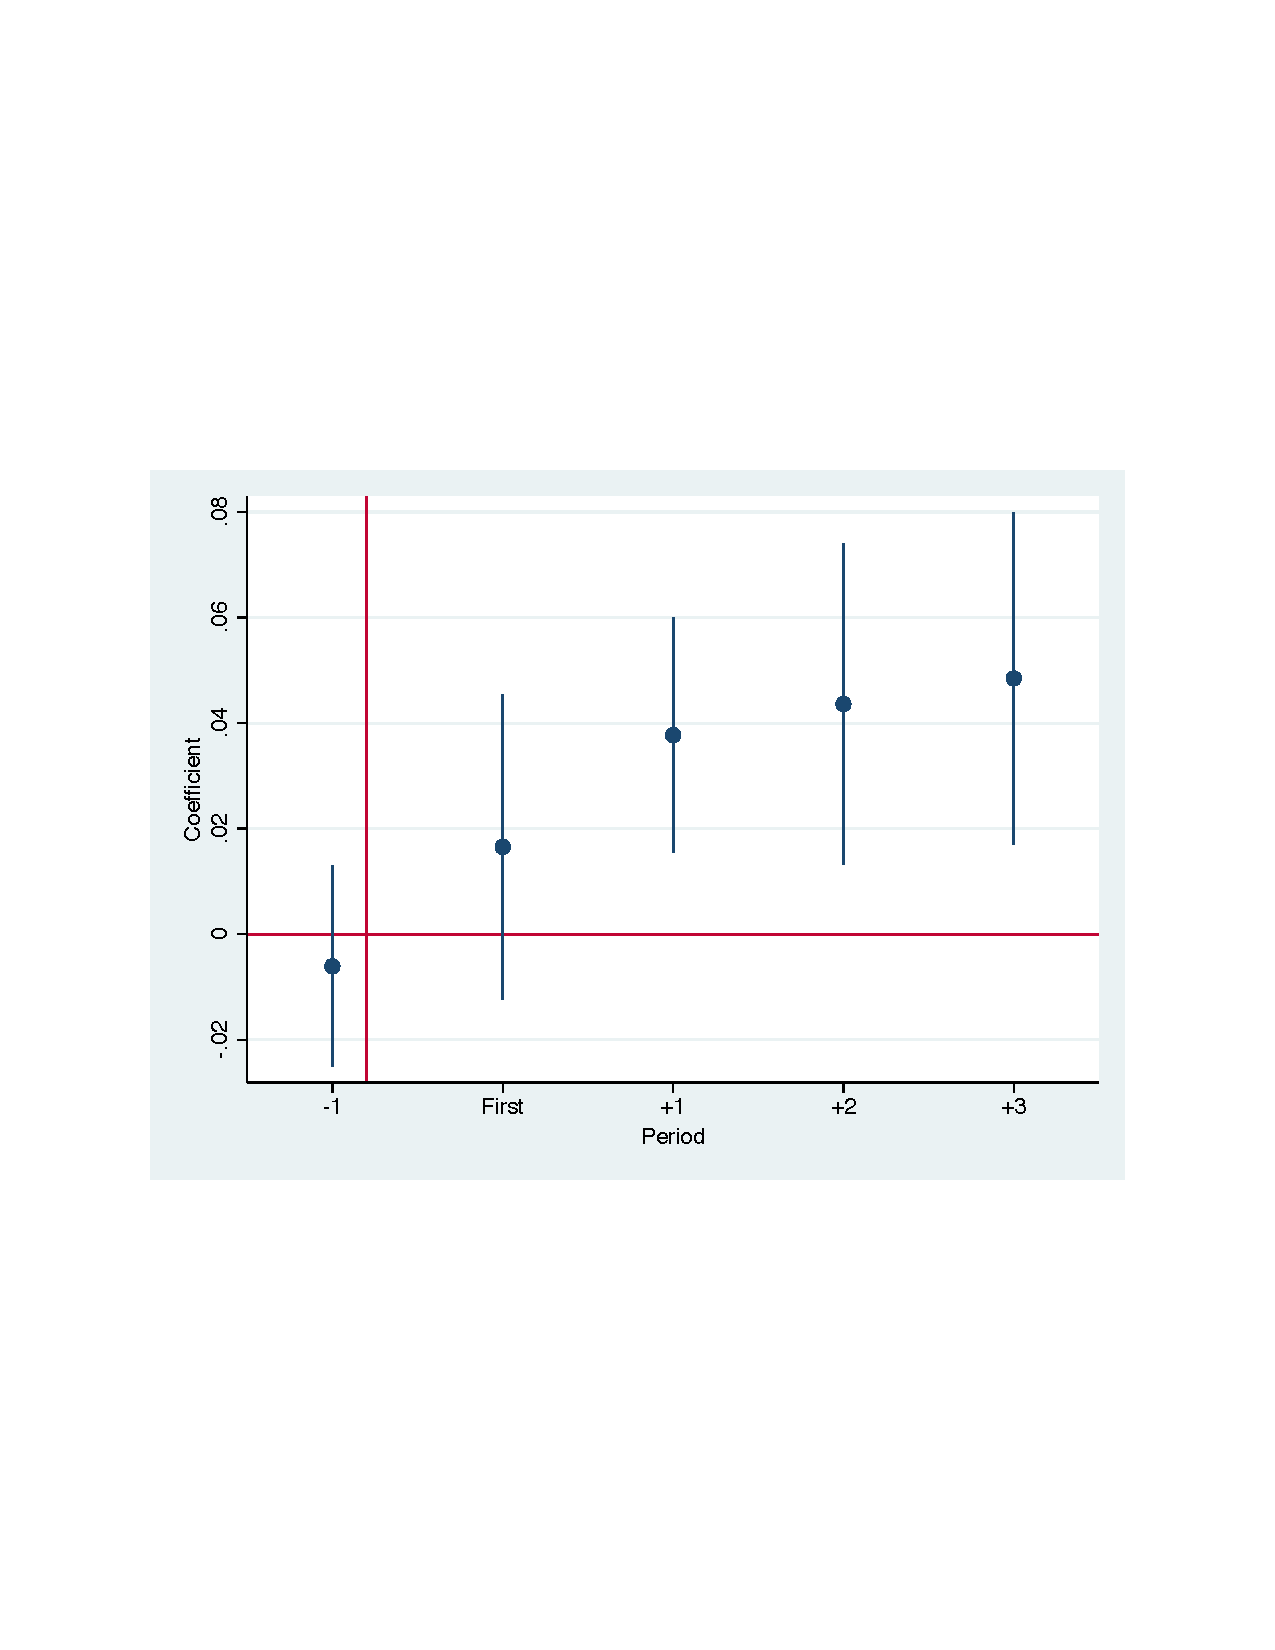
\includegraphics[scale=0.5]{ev_lnprice_hcci_2012.pdf} \\
a.																	& b. \\
\end{tabular}
}
\setlength{\captionmargin}{.5 \textwidth} \addtolength{\captionmargin}{-.5\wd\gfxbox}
\begin{figure}[ht!]
\centering
\caption{Event Study: Log Payments}
\label{fig:event}
\usebox{\gfxbox}
\par
\begin{minipage}{\wd\gfxbox}
\footnotesize
Notes:  Depiction of event study results in which ``first'' represents the first year in which a penalty is realized. Panel a. presents lagged and lead estimates for the entire sample without regard to selection effects (i.e., not all penalized hospitals contribute to the point estimates for each lag/lead).  Panel b. depicts results restricting the sample to just hospitals first penalized in 2012 and those never penalized.
\end{minipage}
\end{figure}

\newpage
\savebox{\gfxbox}{
\centering
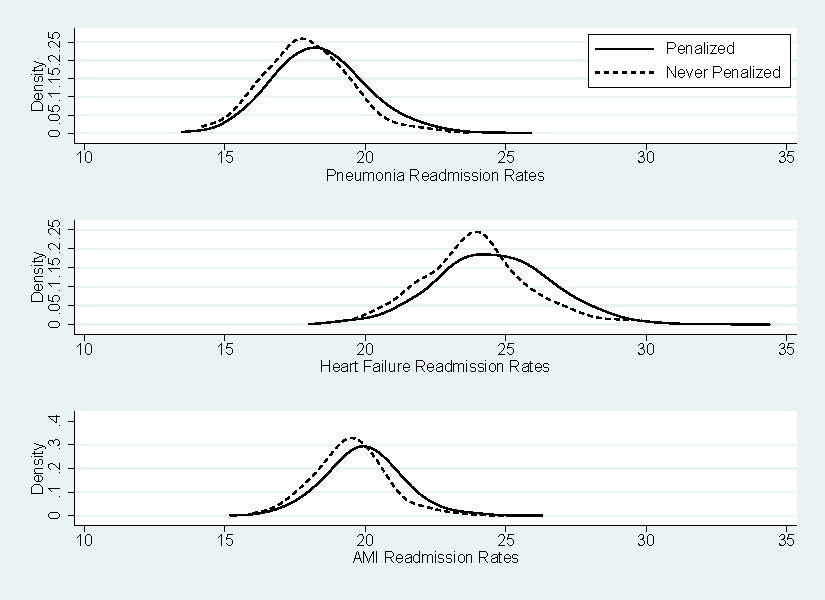
\includegraphics[scale=1]{Readmit_Graphs.pdf}\\
}
\setlength{\captionmargin}{.5 \textwidth} \addtolength{\captionmargin}{-.5\wd\gfxbox}
\begin{figure}[ht!]
\centering
\caption{Pre-HRRP/HVBP Readmission Rates}
\label{fig:pre_readmits}
\usebox{\gfxbox}
\par
\begin{minipage}{\wd\gfxbox}
\footnotesize
Notes:  Kernel density estimates for readmission rates prior to HRRP/HVBP among hospitals ultimately penalized versus those not penalized. Readmission rates reflect reported rates in 2010 and 2011, which are constructed from rates in 2006-2009 and 2007-2010, respectively.
\end{minipage}
\end{figure}

\clearpage

\section*{Tables}
\label{app:tables}


\savebox{\gfxbox}{
\begin{tabular}{ccccccc}
\hline \hline
%\multicolumn{9}{c}{}\\
Fiscal & Sample 	&  Payment $\$$				& Medicare   & Medicaid  	& Other & Percent \\
Year   &  Size    	&  Mean (St. Dev.) 				& Discharges    	& Discharges       	& Discharges   & Penalized \\
 \hline
2010 &      1,386		& 	10,729.22   (4,936.50)	 &   4,614.62  &   2,010.11    &  7,898.18  & 0.00  \\
2011 &      1,386		& 	11,602.74   (5,076.45)	&  4,618.93    & 1,960.05    &  7,892.21  & 0.00   \\
2012 & 	1,386 		& 	12,079.46   (5,567.76) 	  &  4,493.31  &  1,810.27   &   8,019.04  & 0.32   \\
2013 & 	1,386		& 	12,668.44   (5,567.76)	  & 4,396.32    & 1,783.81    &  7,996.10  & 0.74  \\
2014 & 	1,386		&	12,795.83   (5,444.21)	 &    4,260.43   &   1,726.25  &    7,852.71 & 0.76 \\
2015 &    1,386			& 	13,397.63   (5,921.74)	&    4,311.41   &  1,578.86    &   8,261.74 & 0.79 \\
\hline
Total & 	8,316		& 12,212.22   (5,481.55)	  &    4,449.17   &  1,811.56  &   7,986.67 & 0.43 \\
\hline
\end{tabular}
}
\setlength{\captionmargin}{.5 \textwidth} \addtolength{\captionmargin}{-.5\wd\gfxbox}
\begin{table}[!h]
\centering
\caption{Characterization of Research Sample over Time}
\label{tab:summarystats}
\usebox{\gfxbox}
\par
\begin{minipage}{\wd\gfxbox}
\footnotesize
Notes: Balanced panel of hospitals over time between 2010 and 2015.  Payment represents the mean dollar amount paid to a hospital in a year over all acute care admissions.  Penalty is a binary variable for whether the combination of HRRP and HVBP resulted in a net payment reduction. Other discharges denotes all discharges other than Medicare and Medicaid.
\end{minipage}
\end{table}



\newpage
\savebox{\gfxbox}{
\footnotesize
\begin{tabular}{lccc}
\hline \hline
Variable 				& Never 			& Ever  				&   	  \\
		   			&  Penalized    		& Penalized			&    p-value   				\\
 \hline
Log(Payment)			&	9.423	&	9.300	&	0.000	\\
Log(Charge)			&      8.843	&	8.726	& 	0.000	\\
System  Membership      	&	0.768	&	0.784	&	0.352	\\
Non-profit     			&	0.790	&	0.692	&	0.000	\\
Log(Case Mix Index)        	&	0.437	&	0.447	&	0.090	\\
\multicolumn{4}{l}{Local Hospital}\\							
\hspace{0.05in} Monopoly  	&	0.133	&	0.113	&	0.110	\\
\hspace{0.05in} Duopoly    	&	0.282	&	0.156	&	0.000	\\
\hspace{0.05in} Triopoly   	&	0.139	&	0.108	&	0.012	\\
\multicolumn{4}{l}{Market Share}\\							
\hspace{0.05in} Medicare  	&	0.338	&	0.330	&	0.056	\\
\hspace{0.05in} Medicaid    	&	0.110	&	0.125	&	0.000	\\
\hspace{0.05in} Medicare+Medicaid      	&	0.447	&	0.455	&	0.086	\\
\hspace{0.05in} Other     	&	0.553	&	0.545	&	0.086	\\
Total Pop. (1000s)     	&	714	&	1,190	&	0.000	\\
\multicolumn{4}{l}{County Age Distribution}\\							
\hspace{0.05in}[18, 34]      	&	0.240	&	0.239	&	0.504	\\
\hspace{0.05in}[35, 64]   	&	0.393	&	0.393	&	0.947	\\
\hspace{0.05in}$>$65    	&	0.133	&	0.130	&	0.101	\\
\multicolumn{4}{l}{County Race Distribution}\\							
\hspace{0.05in}White     	&	0.795	&	0.734	&	0.000	\\
\hspace{0.05in}Black    	&	0.096	&	0.134	&	0.000	\\
\multicolumn{4}{l}{County Income Distribution}\\							
\hspace{0.05in}$<$ \$50k   	&	0.185	&	0.180	&	0.000	\\
\hspace{0.05in}[\$50k, 75k]   	&	0.126	&	0.123	&	0.000	\\
\hspace{0.05in}[\$100k, 150k]       	&	0.132	&	0.132	&	0.820	\\
\hspace{0.05in}$>$ \$150k   	&	0.095	&	0.101	&	0.007	\\
\multicolumn{4}{l}{County Education Distribution}\\							
\hspace{0.05in}High School Only  	&	0.270	&	0.270	&	0.925	\\
\hspace{0.05in}Bachelor's Only    	&	0.197	&	0.191	&	0.005	\\
\hline
\end{tabular}
}
\setlength{\captionmargin}{.5 \textwidth} \addtolength{\captionmargin}{-.5\wd\gfxbox}
\begin{table}[!h]
\centering
\caption{Hospital Characteristics by Penalties}
\label{tab:bypenalty}
\usebox{\gfxbox}
\par
\begin{minipage}{\wd\gfxbox}
\footnotesize
Notes:  $n=8,316$ Summary statistics are split by whether a hospital is ever observed to receive a net penalty in 2012-2015. Payment represents the mean dollar amount paid to a hospital in a year over all acute care admissions.   County level characteristics are from the American Community Survey.
\end{minipage}
\end{table}

\newpage
\savebox{\gfxbox}{
\scriptsize
\begin{tabular}{llllll}
\hline\hline
 			& Log Mean		& Log Mean			& Log Medicaid 	   	& Log Medicare   		& Log Other  			\\
			& Payment		& 	Net Charge		& Discharges      		& Discharges       	& Discharges        	\\
\hline
Net Penalty  					&	0.014***	&	0.008	&	-0.045**	&	-0.027***	&	-0.004	\\
							&	(0.005)	&	(0.008)	&	(0.021)	&	(0.007)	&	(0.011)	\\
\multicolumn{6}{l}{Hospital Characteristics}\\											
\hspace{0.15in} Monopoly			&	-0.008	&	0.004	&	-0.025	&	0.003	&	-0.012	\\
							&	(0.012)	&	(0.011)	&	(0.055)	&	(0.025)	&	(0.029)	\\
\hspace{0.15in} Duopoly			&	-0.005	&	0.010	&	0.036	&	0.030	&	0.013	\\
							&	(0.010)	&	-(0.010)	&	(0.044)	&	(0.019)	&	(0.023)	\\
\hspace{0.15in} Triopoly			&	0.000	&	0.003	&	-0.000	&	0.002	&	0.006	\\
							&	(0.009)	&	(0.008)	&	(0.039)	&	(0.015)	&	(0.019)	\\
\hspace{0.10in} Large Market		&	-0.041	&	0.001	&	-0.063	&	0.049**	&	0.179***	\\
							&	(0.028)	&	(0.013)	&	(0.050)	&	(0.020)	&	(0.043)	\\
\hspace{0.10in} Any Teaching		&	-0.018	&	-0.022	&	-0.047	&	-0.021	&	-0.013	\\
							&	(0.012)	&	(0.014)	&	(0.039)	&	(0.016)	&	(0.022)	\\
\hspace{0.10in} Major Teaching		&	0.003	&	-0.001	&	0.008	&	0.009	&	0.011	\\
							&	(0.006)	&	(0.004)	&	(0.026)	&	(0.010)	&	(0.012)	\\
\hspace{0.10in} System			&	0.019	&	-0.002	&	-0.091**	&	-0.066***	&	-0.083***	\\
							&	(0.015)	&	(0.011)	&	(0.041)	&	(0.019)	&	(0.020)	\\
\hspace{0.10in} Nonprofit			&	0.020 &	-0.009	&	0.073	&	0.036	&	0.016	\\
							&	(0.026)	&	(0.016)	&	(0.058)	&	(0.028)	&	(0.032)	\\
\multicolumn{6}{l}{County Age Share}\\											
\hspace{0.1in}[18,34]			&	-1.132*	&	-0.896*	&	2.902	&	-3.163***	&	-1.418	\\
							&	(0.681)	&	(0.543)	&	(2.327)	&	(0.853)	&	(0.880)	\\
\hspace{0.1in}[35,64]			&	-0.402	&	-1.182*	&	2.923	&	-3.428***	&	-0.044	\\
							&	(0.910)&	(0.656)	&	(2.781)	&	(1.171)	&	(1.295)	\\
\hspace{0.1in} $>$64			&	-0.488	&	0.281	&	-1.440	&	0.361	&	-0.838	\\
							&	(0.797)	&	(0.671)	&	(2.765)	&	(1.245)	&	(1.359)	\\
\multicolumn{6}{l}{County Share in Race Group}\\											
\hspace{0.1in} Share White		&	-0.321*	&	-0.118	&	-1.165*	&	-0.290	&	0.344	\\
							&	(0.191)	&	(0.156)	&	(0.684)	&	(0.248)	&	(0.313)	\\
\hspace{0.1in} Share Black		&	0.082	&	0.125	&	-1.559	&	-0.396	&	-0.948*	\\
							&	(0.288)	&	(0.263)	&	(1.090)	&	(0.382)	&	(0.498)	\\
\multicolumn{6}{l}{County Share in Income Group}\\											
\hspace{0.1in} 50k-75k			&	-0.288	&	-0.034	&	1.518	&	-0.173	&	0.420	\\
							&	(0.386)	&	(0.286)	&	(1.439)	&	(0.548)	&	(0.790)	\\
\hspace{0.1in} 75k-100k			&	-0.279	&	0.649*	&	0.281	&	-0.319	&	-0.286	\\
							&	(0.479)	&	(0.352)	&	(1.736)	&	(0.623)	&	(0.791)	\\
\hspace{0.1in} 100k-150k			&	-0.736	&	0.290	&	-1.847	&	-0.017	&	0.072	\\
							&	(0.457)	&	(0.313)	&	(1.533)	&	(0.625)	&	(0.776)	\\
\hspace{0.1in}$>$150k			&	0.891**	&	-0.139	&	0.814	&	0.997*	&	-1.767***	\\
							&	(0.402)	&	(0.314)	&	(1.375)	&	(0.511)	&	(0.671)	\\
\hline
\end{tabular}
}
\setlength{\captionmargin}{.5 \textwidth} \addtolength{\captionmargin}{-.5\wd\gfxbox}
\begin{table}[!h]
\centering
\caption{Baseline Results}
\label{tab:baselineresults}
\usebox{\gfxbox}
\par
\begin{minipage}{\wd\gfxbox}
\footnotesize
Notes: $n=8,316$.  All regressions include hospital and year fixed effects and other hospital level controls including bed count and labor force characteristics.  Market power variables are constructed using the overall hospital service area.  Large market is a binary variable for a hospital in the top half of the market size distribution.  In cases in which independent variables are missing, we recode them and control for missing variable indicators to ensure a balanced panel.  Standard errors are clustered at the hospital level.  *** p-value$<$0.01, ** p-value$<$0.05, * p-value$<$0.1.
\end{minipage}
\end{table}






\newpage
\savebox{\gfxbox}{
\scriptsize
\begin{tabular}{llllll}
\hline\hline
 			& Log Mean		& Log Mean			& Log Medicaid 	   	& Log Medicare   		& Log Other  			\\
			& Payment		& 	Net Charge		& Discharges      		& Discharges       	& Discharges        	\\
\hline
Large Bonus	&	-0.005	&	0.017	&	0.022	&	0.026**	&	0.042**	\\
			&	(0.008)	&	(0.012)	&	(0.034)	&	(0.013)	&	(0.017)	\\
\multicolumn{6}{l}{Small Bonus: Omitted Category}\\											
Small Penalty	&	0.010*	&	0.015	&	-0.026	&	-0.017*	&	0.004	\\
			&	(0.006)	&	(0.010)	&	(0.029)	&	(0.010)	&	(0.015)	\\
Large Penalty	&	0.013*	&	0.017	&	-0.047	&	-0.009	&	0.034**	\\
			&	(0.007)	&	(0.012)	&	(0.030)	&	(0.011)	&	(0.016)	\\
\hline
\end{tabular}
}
\setlength{\captionmargin}{.5 \textwidth} \addtolength{\captionmargin}{-.5\wd\gfxbox}
\begin{table}[!h]
\centering
\caption{Intensive Margin Results Results}
\label{tab:int}
\usebox{\gfxbox}
\par
\begin{minipage}{\wd\gfxbox}
\footnotesize
Notes: $n=8,316$.  Results derived from breaking the dollar change in reimbursements above and below the median for those hospitals receiving a bonus and those receiving a penalty, respectively.  All regressions include hospital and year fixed effects and other hospital level controls including bed count and labor force characteristics.  Market power variables are constructed using the overall hospital service area.  Large market is a binary variable for a hospital in the top half of the market size distribution.  In cases in which independent variables are missing, we recode them and control for missing variable indicators to ensure a balanced panel.  Standard errors are clustered at the hospital level.  *** p-value$<$0.01, ** p-value$<$0.05, * p-value$<$0.1.
\end{minipage}
\end{table}























\newpage
\savebox{\gfxbox}{
\footnotesize
\begin{tabular}{llllll}
\hline	
\hline
 			& Log Mean 				& Log Mean			& Log Medicaid 	   	& Log Medicare   		& Log Other  			\\
			& Payment		& 	Net Charge	& Discharges      		& Discharges       	& Discharges    \\
	\hline
\multicolumn{6}{c}{1. Penalty Specific Trends} 											\\
\hline											
Net Penalty 	&	0.010**	&	0.019**	&	-0.038	&	-0.026***	&	-0.011	\\
			&	(0.005)	&	(0.008)	&	(0.023)	&	(0.007)	&	(0.012)	\\
p-value & 0.497 & 0.041 & 0.250 & 0.005 & 0.446 \\
\hline											
\multicolumn{6}{c}{2. Hospital, Year, and County Fixed Effects} 											\\
\hline											
Net Penalty 	&	0.015***	&	0.009	&	-0.048**	&	-0.027***	&	-0.003	\\
			&	(0.005)	&	(0.008)	&	(0.022)	&	(0.007)	&	(0.011)	\\
\hline											
\multicolumn{6}{c}{3. Controlling for Medicaid Expansion States} 											\\
\hline											
Net Penalty 	&	0.014***	&	0.008	&	-0.044**	&	-0.027***	&	-0.005	\\
			&	(0.005)	&	(0.008)	&	(0.021)	&	(0.007)	&	(0.010)	\\
\hline											
\multicolumn{6}{c}{4. Controlling for Overall HCAHPS Hospital Rating} 											\\
\hline											
Net Penalty 	&	0.014***	&	0.008	&	-0.045**	&	-0.026***	&	-0.003	\\
			&	(0.005)	&	(0.008)	&	(0.021)	&	(0.007)	&	(0.010)	\\
\hline											
\multicolumn{6}{c}{5. Dropping Fiscal 2012} 											\\
\hline											
Net Penalty 	&	0.012**	&	0.010	&	-0.045*	&	-0.028***	&	-0.007	\\
			&(0.005)		&	(0.009)		&(0.023)		&(0.007)	&	(0.012)	\\
\hline											
\multicolumn{6}{c}{6. Controlling for Case Mix} 		\\								
\hline											
Net Penalty 	&	0.014***	&	0.004	&	-0.044**	&	-0.026***	&	-0.005	\\
			&(0.005)		&	(0.008)		&(0.021)		&(0.007)	&	(0.011)	\\
\hline
\multicolumn{6}{c}{7. Omitting Hospital Fixed Effects} 		\\								
\hline
Net Penalty 	&	-0.061***	&	-0.049***	&	0.220***	&	0.094***	&	0.069***	\\
			& (0.015)		&	(0.018)		&(0.045)		&(0.026)	&	(0.022)	\\
\hline

\end{tabular}
}
\setlength{\captionmargin}{.5 \textwidth} \addtolength{\captionmargin}{-.5\wd\gfxbox}
\begin{table}[!h]
\centering
\caption{Robustness Checks}
\label{tab:robustness}
\usebox{\gfxbox}
\par
\begin{minipage}{\wd\gfxbox}
\footnotesize
Notes: Further controls include those in our baseline specification for mean payments.  The p-value in the first row of results is in reference to the null hypothesis that trends in the outcome of interest are the same between ever-penalized and never-penalized hospitals conditional on the model covariates.  In cases in which independent variables are missing, we recode them and control for missing variable indicators to ensure a balanced panel.  Standard errors are clustered at the hospital level.  *** p-value$<$0.01, ** p-value$<$0.05, * p-value$<$0.1.
\end{minipage}
\end{table}


\newpage
\savebox{\gfxbox}{
\begin{tabular}{llllll}
\hline	
\hline
 			& Log Mean			& Log Mean				& Log Medicaid 	   	& Log Medicare   		& Log Other  			\\
			& Payment			& Net Charge				& Discharges      		& Discharges       	& Discharges    \\
	\hline
\multicolumn{6}{c}{Non-profit Hospitals}\\											
\hline											
Net Penalty 	&	0.015***	&	0.008	&	-0.046*	&	-0.029***	&	-0.011	\\
			&	(0.005)	&	(0.009)	&	(0.024)	&	(0.007)	&	(0.012)	\\
\hline											
\multicolumn{6}{c}{Non-Profit Hospitals with Penalty Specific Trends} 											\\
						\hline					
Net Penalty 	&	0.012**	&	0.015*	&	-0.039	&	-0.023***	&	-0.015	\\
			&	(0.005)	&	(0.009)	&	(0.026)	&	(0.007)	&	(0.014)	\\
p-value & 0.805 & 0.205 & 0.241 & 0.001 & 0.849 \\
\hline											
\multicolumn{6}{c}{For-profit Hospitals}\\											
\hline											
Net Penalty 	&	0.020	&	0.023	&	-0.018	&	-0.008	&	0.026	\\
			&	(0.014)	&	(0.021)	&	(0.050)	&	(0.018)	&	(0.020)	\\
\hline											
\multicolumn{6}{c}{For-Profit Hospitals with Penalty Specific Trends} 											\\
\hline											
Net Penalty	&	0.011	&	0.043*	&	0.002	&	-0.028	&	0.007	\\
			&	(0.014)	&	(0.023)	&	(0.050)	&	(0.017)	&	(0.020)	\\
p-value & 0.417 & 0.025 & 0.885 & 0.013 & 0.003 \\
\hline
\end{tabular}
}
\setlength{\captionmargin}{.5 \textwidth} \addtolength{\captionmargin}{-.5\wd\gfxbox}
\begin{table}[!h]
\centering
\caption{Results by Profit Status}
\label{tab:byprofit}
\usebox{\gfxbox}
\par
\begin{minipage}{\wd\gfxbox}
\footnotesize
Notes: All regressions include hospital and year fixed effects.  Further controls include those in our baseline specification for mean payments.  The p-values are in reference to the null hypothesis that trends in the outcome of interest are the same between ever-penalized and never-penalized hospitals conditional on the model covariates.  In cases in which independent variables are missing, we recode them and control for missing variable indicators to ensure a balanced panel.  Standard errors are clustered at the hospital level.  *** p-value$<$0.01, ** p-value$<$0.05, * p-value$<$0.1.
\end{minipage}
\end{table}





%\newpage
%\savebox{\gfxbox}{
%\footnotesize
%\begin{tabular}{lllllll}
%\hline	
%\hline
% 			& Log 				& Log				& Medicaid 	   	& Medicare   		& Private  			& Profit  \\
%			& Payment		& Charge			& Discharges      		& Discharges       	& Discharges        	& Index  \\
%\hline
%\multicolumn{7}{c}{Small Markets} \\
%\hline
%Net Penalty	&	0.003	&	-0.007	&	-0.049	&	-0.034*	&	-0.029	&	0.002	\\
%	&	(0.010)	&	(0.015)	&	(0.043)	&	(0.018)	&	(0.022)	&	(0.003)	\\
%\hspace{0.1in} *Med. Mkt. Share 	&	-0.004	&	0.030*	&	0.031	&	0.008	&	0.035	&	-0.003	\\
%	&	(0.012)	&	(0.018)	&	(0.046)	&	(0.020)	&	(0.024)	&	(0.004)	\\
%\hspace{0.1in} *High Mkt. Share 	&	0.009	&	-0.004	&	-0.002	&	0.014	&	0.030	&	0.000	\\
%	&	(0.012)	&	(0.019	)&	(0.051)	&	(0.022)	&	(0.024)	&	(0.004)	\\	
%Market Share	&	0.009	&	-0.056**	&	0.167**	&	0.216***	&	0.321***	&	0.004	\\
%\hspace{0.1in} Medium	&	(0.011)	&	(0.026)	&	(0.080)	&	(0.038)	&	(0.049)	&	(0.004)	\\
%Market Share	&	0.012	&	-0.047	&	0.294***	&	0.288***	&	0.428***	&	0.004	\\
%\hspace{0.1in} High	&	(0.017)	&	(0.035)	&	(0.102)	&	(0.054)	&	(0.063)	&	(0.006)	\\
%\hline
%\multicolumn{7}{c}{Large Markets} \\
%\hline
%Net Penalty	&	0.036***	&	-0.001	&	-0.072*	&	-0.022	&	0.010	&	0.000	\\
%	&	(0.012)	&	(0.018)	&	(0.040)	&	(0.018)	&	(0.025)	&	(0.003)	\\
%\hspace{0.1in} *Med. Mkt. Share 	&	-0.013	&	0.018	&	0.046	&	0.018	&	0.019	&	0.006*	\\
%	&	(0.013)	&	(0.018)	&	(0.038)	&	(0.018)	&	(0.022)	&	(0.003)	\\
%\hspace{0.1in} *High Mkt. Share	&	-0.022*	&	0.038*	&	0.051	&	0.024	&	-0.003	&	0.002	\\
%	&	(0.013)	&	(0.020)	&	(0.039)	&	(0.019)	&	(0.025)	&	(0.003)	\\	
%Market Share	&	-0.001	&	-0.049**	&	0.364***	&	0.360***	&	0.395***	&	-0.003	\\
%\hspace{0.1in} Medium	&	(0.016)	&	(0.021)	&	(0.057)	&	(0.047)	&	(0.060)	&	(0.005)	\\
%Market Share	&	0.009	&	-0.138***	&	0.515***	&	0.513***	&	0.688***	&	-0.005	\\
%High 	&	(0.019)	&	(0.032)	&	(0.082)	&	(0.065)	&	(0.097)	&	(0.007)	\\
%
%\hline
%\end{tabular}
%}
%\setlength{\captionmargin}{.5 \textwidth} \addtolength{\captionmargin}{-.5\wd\gfxbox}
%\begin{table}[!h]
%\centering
%\caption{Triple Differences by Market Share}
%\label{tab:bymktshare}
%\usebox{\gfxbox}
%\par
%\begin{minipage}{\wd\gfxbox}
%\footnotesize
%Notes: All regressions include hospital and year fixed effects. Further controls include those in our baseline specification for mean payments.  In cases in which independent variables are missing, we recode them and control for missing variable binary variables to ensure a balanced panel.  We split the sample by market size because of the strong negative correlation between market size and market share. Standard errors are clustered at the hospital level.  *** p-value$<$0.01, ** p-value$<$0.05, * p-value$<$0.1.
%\end{minipage}
%\end{table}




\newpage
\savebox{\gfxbox}{
\footnotesize
\begin{tabular}{lll}
\hline	
 		& Log Mean & Log Mean   				 \\
		& Payment & Net Charge\\
\hline
Net Penalty				&	0.039***	&	0.043***	\\
						&	(0.010)	&	(0.013)	\\
\hspace{0.1in}* Public Share 2 	&	-0.020*	&	-0.014	\\
						&	(0.012)	&	(0.014)	\\
\hspace{0.1in}* Public Share 3	&	-0.033**	&	-0.043***	\\
						&	(0.013)	&	(0.015)	\\
\hspace{0.1in}* Public Share 4	&	-0.044***	&	-0.070***	\\
						&	(0.013)	&	(0.016)	\\
Public Share 2				&	0.007	&	0.049***	\\
						&	(0.010)	&	(0.013)	\\
Public Share 3				&	0.016	&	0.087***	\\
						&	(0.011)	&	(0.016)	\\
Public Share 4				&	0.023*	&	0.157***	\\
						&	(0.012)	&	(0.018)	\\
\hline
\end{tabular}
}
\setlength{\captionmargin}{.5 \textwidth} \addtolength{\captionmargin}{-.5\wd\gfxbox}
\begin{table}[!h]
\centering
\caption{Triple Differences by Public Share}
\label{tab:publicshare}
\usebox{\gfxbox}
\par
\begin{minipage}{\wd\gfxbox}
\footnotesize
Notes: All regressions include hospital and year fixed effects.  Further controls include those in our baseline specification for mean payments.  The share of a hospital's patients insured by the public sector is broken into quartiles and interacted with penalty variables.  In cases in which independent variables are missing, we recode them and control for missing variable indicators to ensure a balanced panel.  Standard errors are clustered at the hospital level.  We restrict the sample to include at least 25 admissions per hospital per year.  *** p-value$<$0.01, ** p-value$<$0.05, * p-value$<$0.1.
\end{minipage}
\end{table}




\newpage
\savebox{\gfxbox}{
\footnotesize
\begin{tabular}{llllll}
\hline	
\hline
 & Log Mean 				& Log Mean			& Log Medicaid 	   	& Log Medicare   		& Log Other  			\\
			& Payment		& 	Net Charge	& Discharges      		& Discharges       	& Discharges    \\
\hline
\multicolumn{6}{c}{Hospitals Integrated Vertically with Physician Groups Prior to 2012} 											\\
\hline											
Net Penalty 	&	0.023***		&	0.017***	&	-0.036	&	-0.026**	&	0.008	\\
			&	(0.008)		&	(0.006)		&(0.032)		&(0.009)	&	(0.016)	\\
			\hline
\multicolumn{6}{c}{Hospitals Never Observed to be Vertically Integrated with a Physician Group} 											\\
\hline											
Net Penalty 	&	0.008		&	0.021***	&	-0.063**	&	-0.024**	&	-0.005	\\
			&	(0.007)		&	(0.012)		&(0.031)		&(0.010)	&	(0.015)	\\
			\hline
\end{tabular}
}
\setlength{\captionmargin}{.5 \textwidth} \addtolength{\captionmargin}{-.5\wd\gfxbox}
\begin{table}[!h]
\centering
\caption{Vertical Integration and Penalties}
\label{tab:VI}
\usebox{\gfxbox}
\par
\begin{minipage}{\wd\gfxbox}
\footnotesize
Notes: Empirical models are identical to those in Table \ref{tab:baselineresults}.  Standard errors are clustered at the hospital level.  *** p-value$<$0.01, ** p-value$<$0.05, * p-value$<$0.1.
\end{minipage}
\end{table}


%> MDC reference:
%> 0 - all admissions
%> 1 - Nervous system
%> 4 - Respiratory system
%> 5 - Circulatory system
%> 8 - Musculoskeletal system and connective tissue
%> 14 - Pregnancy, childbirth, puerperium
%> 15 - Newborns and other neonates

\newpage
\savebox{\gfxbox}{
\begin{tabular}{ccccccc}
\hline	
\hline
 							& Nervous  	& Respiratory  	 & Circulatory    & Musculoskeletal   		& Labor and & Neonatal \\
							&  System		&  System      	&  System     	&  System        			& Delivery   &	\\
\hline
Net Penalty 					& 0.021***		&	0.001 	&	0.019**	&	0.004	&	-0.001	&	0.016	\\
							& (0.010)		&	(0.011)	&	(0.008)	&	(0.007)	&	(0.005)	&	(0.010)	\\
\hline
n							& 1,410		&	1,758 	&	2,754  	&	3,060  	&	5,226	&	3,204	\\
Mean 						&13,762.86	&	12,015.13	&	13,071.17	&	12,981.58	&	11,308.56	&	8,911.19	\\
\hline
\end{tabular}
}
\setlength{\captionmargin}{.5 \textwidth} \addtolength{\captionmargin}{-.5\wd\gfxbox}
\begin{table}[!h]
\centering
\caption{Log Payments for Condition Specific Admissions}
\label{tab:eachcondition}
\usebox{\gfxbox}
\par
\begin{minipage}{\wd\gfxbox}
\footnotesize
Notes: All regressions include hospital and year fixed effects.  The dependent variable is the log of average payments for each associated acute care admission.  Further controls include those in our baseline specification for mean payments.  In cases in which independent variables are missing, we recode them and control for missing variable indicators to ensure a balanced panel.  Standard errors are clustered at the hospital level.  We restrict the sample to include at least 25 admissions per hospital per year.  *** p-value$<$0.01, ** p-value$<$0.05, * p-value$<$0.1.
\end{minipage}
\end{table}




\newpage
\savebox{\gfxbox}{
\footnotesize
\begin{tabular}{llll}
\hline\hline
 				& Profit Index 	& Average DRG 	& Average        	\\
 				& 			& Weight 			& LOS			\\
\hline
\hline							
Net Penalty  		&	0.002	&	0.004	&	0.015 \\
				&	(0.001)	&	(0.004)	&	(0.012)	\\
															
\hline
\end{tabular}
}
\setlength{\captionmargin}{.5 \textwidth} \addtolength{\captionmargin}{-.5\wd\gfxbox}
\begin{table}[!h]
\centering
\caption{Other Results}
\label{tab:other_results}
\usebox{\gfxbox}
\par
\begin{minipage}{\wd\gfxbox}
\footnotesize
Notes: $n=8,316$.  All regressions include hospital and year fixed effects and other hospital level controls include bed count and labor force.  Market power variables are constructed as the overall county market share tercile.  Large market is a binary variable for a hospital in the top half of the market size distribution.  In cases in which independent variables are missing, we recode them and control for missing variable indicators to ensure a balanced panel.  Standard errors are clustered at the hospital level.  *** p-value$<$0.01, ** p-value$<$0.05, * p-value$<$0.1.
\end{minipage}
\end{table}


















\end{document}
